\begin{refsection}
\chapter{Characterisation of Laser Processed Phosphorous Doped Diamond}
\section{Introduction}
\subsection{Summary of Previous Experimental Work}
Chapter \ref{ch:electrical_experiments} examines the formation of conventional metal contacts to heavily phosphorous doped diamond, via annealed titanium-based contacts. The literature best-case value for the specific contact resistivity with titanium contacts is $10^{-3}$~\si{\ohm\centi\metre\squared} \cite{matsumoto2013}. The contacts formed in this work, both in the CTLM and LTLM experiments and under different annealing conditions, differ markedly from these examples. With LTLM samples, the specific contact resistivity was measured to be 472 and 494\si{\kilo\ohm\centi\metre\squared}, with a resistivity of the phosphorous doped film of 132 and 464~\si{\mega\ohm\centi\metre} for samples C and D respectively at 10 V. For sample F and the CTLM results, at a constant current condition of -100 \si{\nano\ampere}, a specific contact resistivity of around 2.1~\si{\kilo\ohm\centi\metre\squared} and resistivity of around 490~\si{\kilo\ohm\centi\metre} was measured. Following these observations, it was clear that an alternative approach must be taken to form superior ohmic contacts on these samples which are sufficient to allow for competitiveness between diamond based power devices and current best case values on standard materials. For example, SiC is able to achive extremely low resistance ohmic contacts below $1\times10^{-7}$~\si{\ohm\centi\metre\squared} \cite{pan2013}.

\subsection{Improved Contacts to Diamond Devices}
Novel approaches to the formation of ohmic contacts with n-type diamond are an ongoing area of research, with unique orientation and substrate dependent methodologies being developed. For instance, \cite{temahuki2017} demonstrated the ability of Ni-catalysed etching to provide pyramidal \hkl(111) oriented pits for a heavily phosphorous doped overgrowth layer. This method provides both geometrically enhanced emitter-type structures, as well as a greater phosphorous concentration than what is otherwise obtainable on a \hkl(100) oriented substrate, hence producing significantly improved contacts than other contacts to n-type \hkl(100) substrates without micro-structures. For \hkl(111) oriented substrates, the results of various metal contact formations are summarised in (reference to comparison of metal contacts on phosphorous doped diamond). While much work in this area treats these metal contacts as ohmic in nature due solely to the nature of the heavy n-type doping and subsequent formation of titanium carbide contacts, unique approaches to further reducing this specific contact resistivity can be seen in \cite{matsumoto2013} and \cite{valappil2022, valappil2023}. In the first such case, thermal graphitisation of the diamond surface is used to provide an additional intermediate layer for the formation of ohmic contacts, achieving an order of magnitude reduction in the specific contact resistivity when compared to the titanium carbide contacts \cite{matsumoto2013}. In the more recent work by Valappil et al, coaxial arc plasma deposition (CAPD) is used to form nanocarbon electrodes which show a similar order of magnitude improvement over the conventional titanium contacts.

One technique that has not yet been utilised for the reduction in specific contact resistivity on heavily phosphorous doped diamond is that of laser processing for the purpose of graphitisation. Laser processing offers numerous advantages over the procedures of nanocarbon CAPD, or thermal graphitisation, such as the ability to directly pattern working contacts without standard photolithography steps, the ability to write 3D structures such as wires passing through the diamond substrate for diamond detectors \cite{bloomer2020}, and the ability to also create waveguides within the diamond substrates through modification of the local refractive index \cite{courvoisier2016}. While unrelated to power electronic applications, it is also worth noting that this process can also be used to generate point defects within diamond substrates, which can be used to generate single negatively charged nitrogen-vacancy (NV$^{-}$) centres, and have a wide array of potential applications in magnetometry, single photon sources, quantum centres, etc. \cite{chen2016}. The combination, or specific usage of any of these key features allows for a large range of device structures to be fabricated by laser graphitisation processes. For a complete review of laser graphitisation, please see chapter \ref{sec:laser}.

\subsection{Field Effect Emission}
\label{subsec:field_effect_emission}
A device structure that may particularly benefit from 3D laser graphitisation is that of the cold-cathode type structure. As described in the seminal work \cite{spindt1976}, it is possible to induce cold-field effect emission with sufficiently sharp (geometrically enhanced) structures. This structure was then proposed to be used in conjunction with the negative electron affinity of hydrogen-terminated diamond \cite{geis1996}, allowing for lower applied voltages to generate practical electron sources that could compete with thermionic emitters. Significant issues with this design structure arise during the fabrication of such structures, due in large part to the etching process and overgrowth of heavily n-type diamond. Parallels could be drawn between the fabrication of these structures and the work of \cite{temahuki2017}, where a random distribution of Ni-etched pits are overgrown with heavily phosphorous doped diamond, and finally contacted with standard Ti/Au contacts. However, the fabrication of emitters as in Geis et al. requires the emitters to be fabricated such that the tips are perpendicular and very close to the surface of the diamond emitters. Any spacing between the tip of the cathode-emitter and the hydrogen terminated diamond surface will result in a large potential difference drop between the cathode and the anode, reducing the effective field strength at the tip and hence significantly affecting the field effect emission of such a device. In practice, this narrow spacing is extremely difficult to achieve via etching, as dislocations or other defects in the diamond substrate will generate fault lines for the etching process, drastically altering the etching rate. Several alternative approaches have been attempted in recent history. Significantly, several devices have been suggested which attempt to either create sharp diamond cathodes \cite{davidson2007diamond}, etching back substrates \cite{sakuma2000manufacturing}, or utilising designs that allow for carbon nanotubes to be employed. There is a notable overlap in device designs that attempt to fabricate emitters based on diamond and graphite \cite{ono2008cold, sakai2004cold}, carbon nanotubes \cite{dimitrijevic2005diamond}, diamond-like carbon layers \cite{goel2002electrically}, amorphous carbon \cite{falabella2001amorphous}, or diamondoid monolayers \cite{yang2013diamondoid}, all of which were designed prior to the development of 3D laser graphitisation processes. Ultimately, all such devices present insufficient properties or flaws, and this area of research is ongoing.

\subsection{Laser Written Geometrically Enhanced Emitters}
A natural proposition for 3D micron scaled laser graphitised wires within diamond such as that demonstrated within \cite{sun2014} is that of cold-cathode type devices. While a practical device that can compete with either one of the aforementioned designs or silicon-based devices is ambitious, as the phosphorous doped CVD growth of diamond and the laser graphitisation processes continue to mature, future devices which make use of these capabilities to generate cold-cathode structures with only one laser processing step may start to appear achievable. This would eliminate the need for many of the processing steps such as the deposition of Ti-C based ohmic contacts, or the need for various etching steps and differing metal depositions to produce sufficient gate electrodes in the triode structure. It also addresses the issue of thin electronic grade diamond samples being required for a suitably narrow region between the emitters and the hydrogen terminated diamond surface, which brings about a host of practical processing concerns. Also note that the requirement of electronic grade diamond for carefully controlled, reliable etching procedures is also tentatively eliminated, as the priority can instead be given to high quality phosphorous doped diamond substrates, benefiting the reduction of Schottky barrier height at the graphite/diamond interface.

Hence, experimental work was planned to examine both the effect of laser processing for the purpose of reduced specific contact resistivity ohmic contacts, and to also explore the possibility of laser written structures utilising an emitter type design.

\subsection{Laser Graphitised Device Design}

\begin{figure}[H]
    \centering
    \includegraphics[width=\textwidth]{Chapter7/Figs/Raster/overview of design.png}
    \caption{An overview of the laser graphitisation design, including alignment markers for potential photolithography steps and various device structures as described in this section.}
    \label{fig:design_overview}
\end{figure}

To test the reduction of specific contact resistivity via laser processing and the preliminary concept of laser graphitised emitters, the laser graphitisation layout as shown in figure \ref{fig:design_overview} was designed. Various strategies were employed to allow for the testing of various specific features. Of particular note are the LTLM structures, CTLM structures and the emitter array seen as an array of rectangular contacts. This allowed for some redundancy in the devices, and the direct comparison between different devices. The best example of this is between the LTLM array, which is a simple rectangular arrangement of contacts with channel spacings between 2--9~\si{\micro\metre}, and the emitter arrays, which had similar rectangular contacts to the LTLM array, but with protruding emitters between the two contacts. The comparison between planar contacts and these geometrically enhanced contacts can then be compared to look for signs of field effect emission due to the sharp emitter features.

\begin{figure}[h]
    \centering
    \includegraphics[width=\textwidth]{Chapter7/Figs/Raster/zoom1 LTLM area.png}
    \caption{A close up of the LTLM design, including scale measurements of relevant feature sizes for clarity.}
    \label{fig:design_ltlm }
\end{figure}

\section{Laser Graphitisation Fabrication}
Laser graphitisation of diamond surfaces allows for significant advancement in the fabrication of diamond-based electronic devices. This technique leverages focused laser beams to convert specific regions of the diamond substrate into graphitic material, facilitating the creation of conductive pathways and contacts essential for device functionality. Precise control over the graphitisation process enables the fabrication of complex structures, such as wires and contact pads, with tailored electrical properties. For a full review of this technique, see chapter \ref{sec:laser}. The laser fabrication of the following sample as tested in this chapter was performed at Oxford University in collaboration with Patrick Salter and Ravi Shivaraman, using the mask designed by the candidate.

\subsection{Laser Fabrication Processing}
The laser graphitisation process employs a state-of-the-art Pharos laser system, operating at a wavelength of 515~\si{\nano\metre}. This system is characterised by its high repetition rate of 10~\si{\kilo\hertz}, which is crucial for achieving consistent graphitisation across the targeted areas. The choice of objective lens and the adjustment of laser pulse energy play significant roles in defining the morphology and conductivity of the graphitised structures.

\subsubsection{Laser Parameters and Setup} 
The fabrication of graphitic wires and contact pads utilised objective lenses with numerical apertures (NA) of 0.75 and 0.5, respectively. The higher pulse energy facilitated by the 0.75 NA objective lens is preferred for creating wider wires, while the 0.5 NA lens is suited for processing the contact pads. Notably, the sequence in which these components are fabricated; starting with the contact pads before the wires, was observed during initial processing to influence the wire morphology, particularly near the pads. This suggests that the local thermal and structural changes induced by the pad fabrication can affect subsequent graphitisation steps.

\subsubsection{Calibration of Pulse Energy} 
The precise calibration of pulse energy is critical for optimising the graphitisation process. Although initial settings were based on angular adjustments of the waveplate, detailed calibration is necessary to correlate these settings with specific pulse energies. This calibration ensures that the laser energy delivered to the diamond surface is precisely controlled, minimising damage to surrounding areas while maximising the quality and conductivity of the graphitic structures.

\subsubsection{Significance of Laser Processing Parameters} 
\label{subsubsec:significance_of_laser_processing_parameters}
The choice of laser parameters, including the repetition rate, pulse energy, and objective lens, directly impacts the efficiency and outcome of the graphitisation process. These parameters determine the depth, width, and electrical properties of the graphitic structures, influencing the performance of the final diamond-based devices. It is also important to note that the sample used here is different to that found in previous studies \cite{sun2014}, \cite{salter2024}, the samples are \hkl(111) oriented HPHT substrates, with a highly phosphorous doped surface layer of $\sim1.2$~\si{\micro\metre} thickness, whereas work in the literature is performed on \hkl(100) oriented, undoped CVD substrates.

This subsection has outlined the foundational aspects of the laser graphitisation fabrication process, highlighting the critical role of laser parameters in achieving desired structural and electrical characteristics. Further characterisation techniques, such as AFM, PL, and Raman spectroscopy, provide deeper insights into the quality and properties of the graphitised diamond, which will be discussed in the subsequent sections.

\subsection{AFM Characterisation}
\label{subsec:afm_characterisation}
To characterise the surface topology of the laser graphitised devices, AFM was used to provide broad overviews of the resulting structures following the fabrication at Oxford. 

\begin{figure}[H]
    \centering
    \includegraphics[width=\textwidth]{Chapter7/Figs/Raster/21 meh 4k_white_annotated_downscaled.jpg}
    \caption{A large area AFM scan of the LTLM channel that was designed to have a spacing of 2~\si{\micro\metre}.}
    \label{fig:afm_21_big}
\end{figure}

Figure \ref{fig:afm_21_big} shows a broad scan of the LTLM contacts that were designed to have a spacing of 2~\si{\micro\metre}. The top left corner of this scan experienced a systematic error, visible as a raised blur. Preliminary low resolution scans of this region did not contain this error, and it can hence be identified as a scanning error unrelated to the sample. Otherwise, the scan managed to achieve a generally high level of detail, despite the 90~\si{\micro\metre} square area being close to the maximum scan area for the XE-150 system. Of note is the slightly inconsistent channel length between the two rectangular contacts, presented in the exact centre of the figure. At the top and bottom of the contacts, marked by the green capsules, the channel is visibly squeezed in, with the rest of the channel presenting a thicker separation. It is also possible to see that the laser graphitisation has etched down into the diamond surface on the order of 1~\si{\micro\metre}. This presented a concern that the laser graphitisation process may have etched through the active, phosphorous doped layer of $1.2$~\si{\micro\metre}, with thin graphite walls on the edges of the ablated regions providing electrical contact, in contrast to the intended block of graphitic material in full proximity to the phosphorous doped channel.

\begin{figure}[H]
    \centering
    \includegraphics[width=\textwidth]{Chapter7/Figs/Raster/bone_scan_whiteh_downscaled.jpg}
    \caption{A large area AFM scan of the wider graphitised surface wire, with adjacent contacts for emitter array testing.}
    \label{fig:afm_bone}
\end{figure}

Figure \ref{fig:afm_bone} displays a portion of the control surface wire that was included in the graphitisation design for calibration purposes. This surface wire had a designed thickness of 14~\si{\micro\metre}, to allow for preliminary testing of the written graphite resistivity. While this large scale AFM scan suffers from some noise in the centre of the scan region, it does provide another view of the as written structures, and how they deviate from the design with specific topological features apparent on the sides of the contact wires. The laser written contacts are observed to be up to approximately 2~\si{\micro\metre} deep relative to the diamond surface, with steep walls at the side of the written trenches.
\clearpage
\subsubsection{Trench Wall Steepness and AFM Tip Profile}
\label{subsubsec:trench_wall_steepness}

\begin{wrapfigure}{r}{0.5\textwidth} % 'r' for right, 'l' for left; and the width of the figure.
  \centering
  \includegraphics[width=0.48\textwidth]{Chapter7/Figs/Raster/ACTA tip.png}
  \caption{An SEM scan of a typical ACTA tip, as provided in the technical specifications sheet by Applied NanoStructures Inc.}
  \label{fig:acta_tip}
\end{wrapfigure}

It is important to note one detail in particular of the AFM scans, that of the graphitised trench steepness, or the profile of the trench walls. For the purpose of examining the large area AFM scans, it is necessary to consider more precisely the observed steepness of the written contacts and the possible impact of the AFM tip itself. Figure \ref{fig:acta_tip} shows a typical ACTA probe as were used in these scans, utilising a rectangular Si cantilever, a pyramidal tip of height $14$--$16$~\si{\micro\metre} and radius of curvature $6$~\si{\micro\metre}. The exact dimensions of the AFM tip may differ from probe to probe, but the pyramidal tip may have had some impact on the observed steepness of etched trenches due to the widening of the base away from the tip.

In NC-AFM, D-AFM or C-AFM, when the tip passes from the diamond surface into the trench, it will quickly descend, with the rate of descent determined primarily by the chosen drive in the Z-scanner. This is then recorded as an incline and less steep wall, with the exact slope being determined by the scan rate if the tip is in relative free-fall after leaving the diamond surface. Equally, when the tip is instead passing from the trench and encounters the trench wall, it may detect the wall itself well beyond the point of the tip coming into contact, due to the pyramidal base meeting the wall first. The piezoelectric system will hence raise the tip, as it detects the side wall with the pyramidal base as for the tip. In this situation, the scan rate may also lead to the risk of direct collision between the pyramidal base and the sidewall, ultimately leading to damage of the AFM tip.

\begin{figure}[H]
    \centering
    \includegraphics[width=\textwidth]{Chapter7/Figs/Raster/jet_legend_um.png}
    \caption{A comparison of three different NC-AFM scan rates on a laser graphitised trench structure. The data are planarised based on the first and last data points, to represent the estimated diamond surface level.}
    \label{fig:afm_scan_rate_small}
\end{figure}

Figure \ref{fig:afm_scan_rate_small} has a few notable features which demonstrate this process when using NC-AFM. First, all three scan rates have distinct peaks and troughs as they pass through the laser graphitised channels. The sharp, triangular troughs perhaps directly reflect the triangular AFM tip in action when it meets a sharp drop in the z-axis. Second, it is clear that the direction of the scan impacts the observed edges of the graphitised trenches. In this figure, the scan is passing from the left to the right. While the first trench appears to have a relatively low slope, with agreement between all three scan rates, the descent into the second trench has a notable discrepancy between the two lower scan rates and the highest included scan rate of $15$~\si{\micro\metre\per\second}. In contrast, the walls as seen by the ascending AFM tip are in relative agreement, as they all encounter the wall and must ascend very quickly to ensure that the tip does not impact the wall. It is also notable that the observed trench depth decreases as a function of the AFM scan rate, indicating that at the lowest scan rates the system is better recognising the correct altitude of the tip, as it has time to adjust based on the specific features within the channels.

\subsubsection{Further AFM Scans}
\label{subsubsec:further_afm_scans}

\begin{figure}[H]
    \centering
    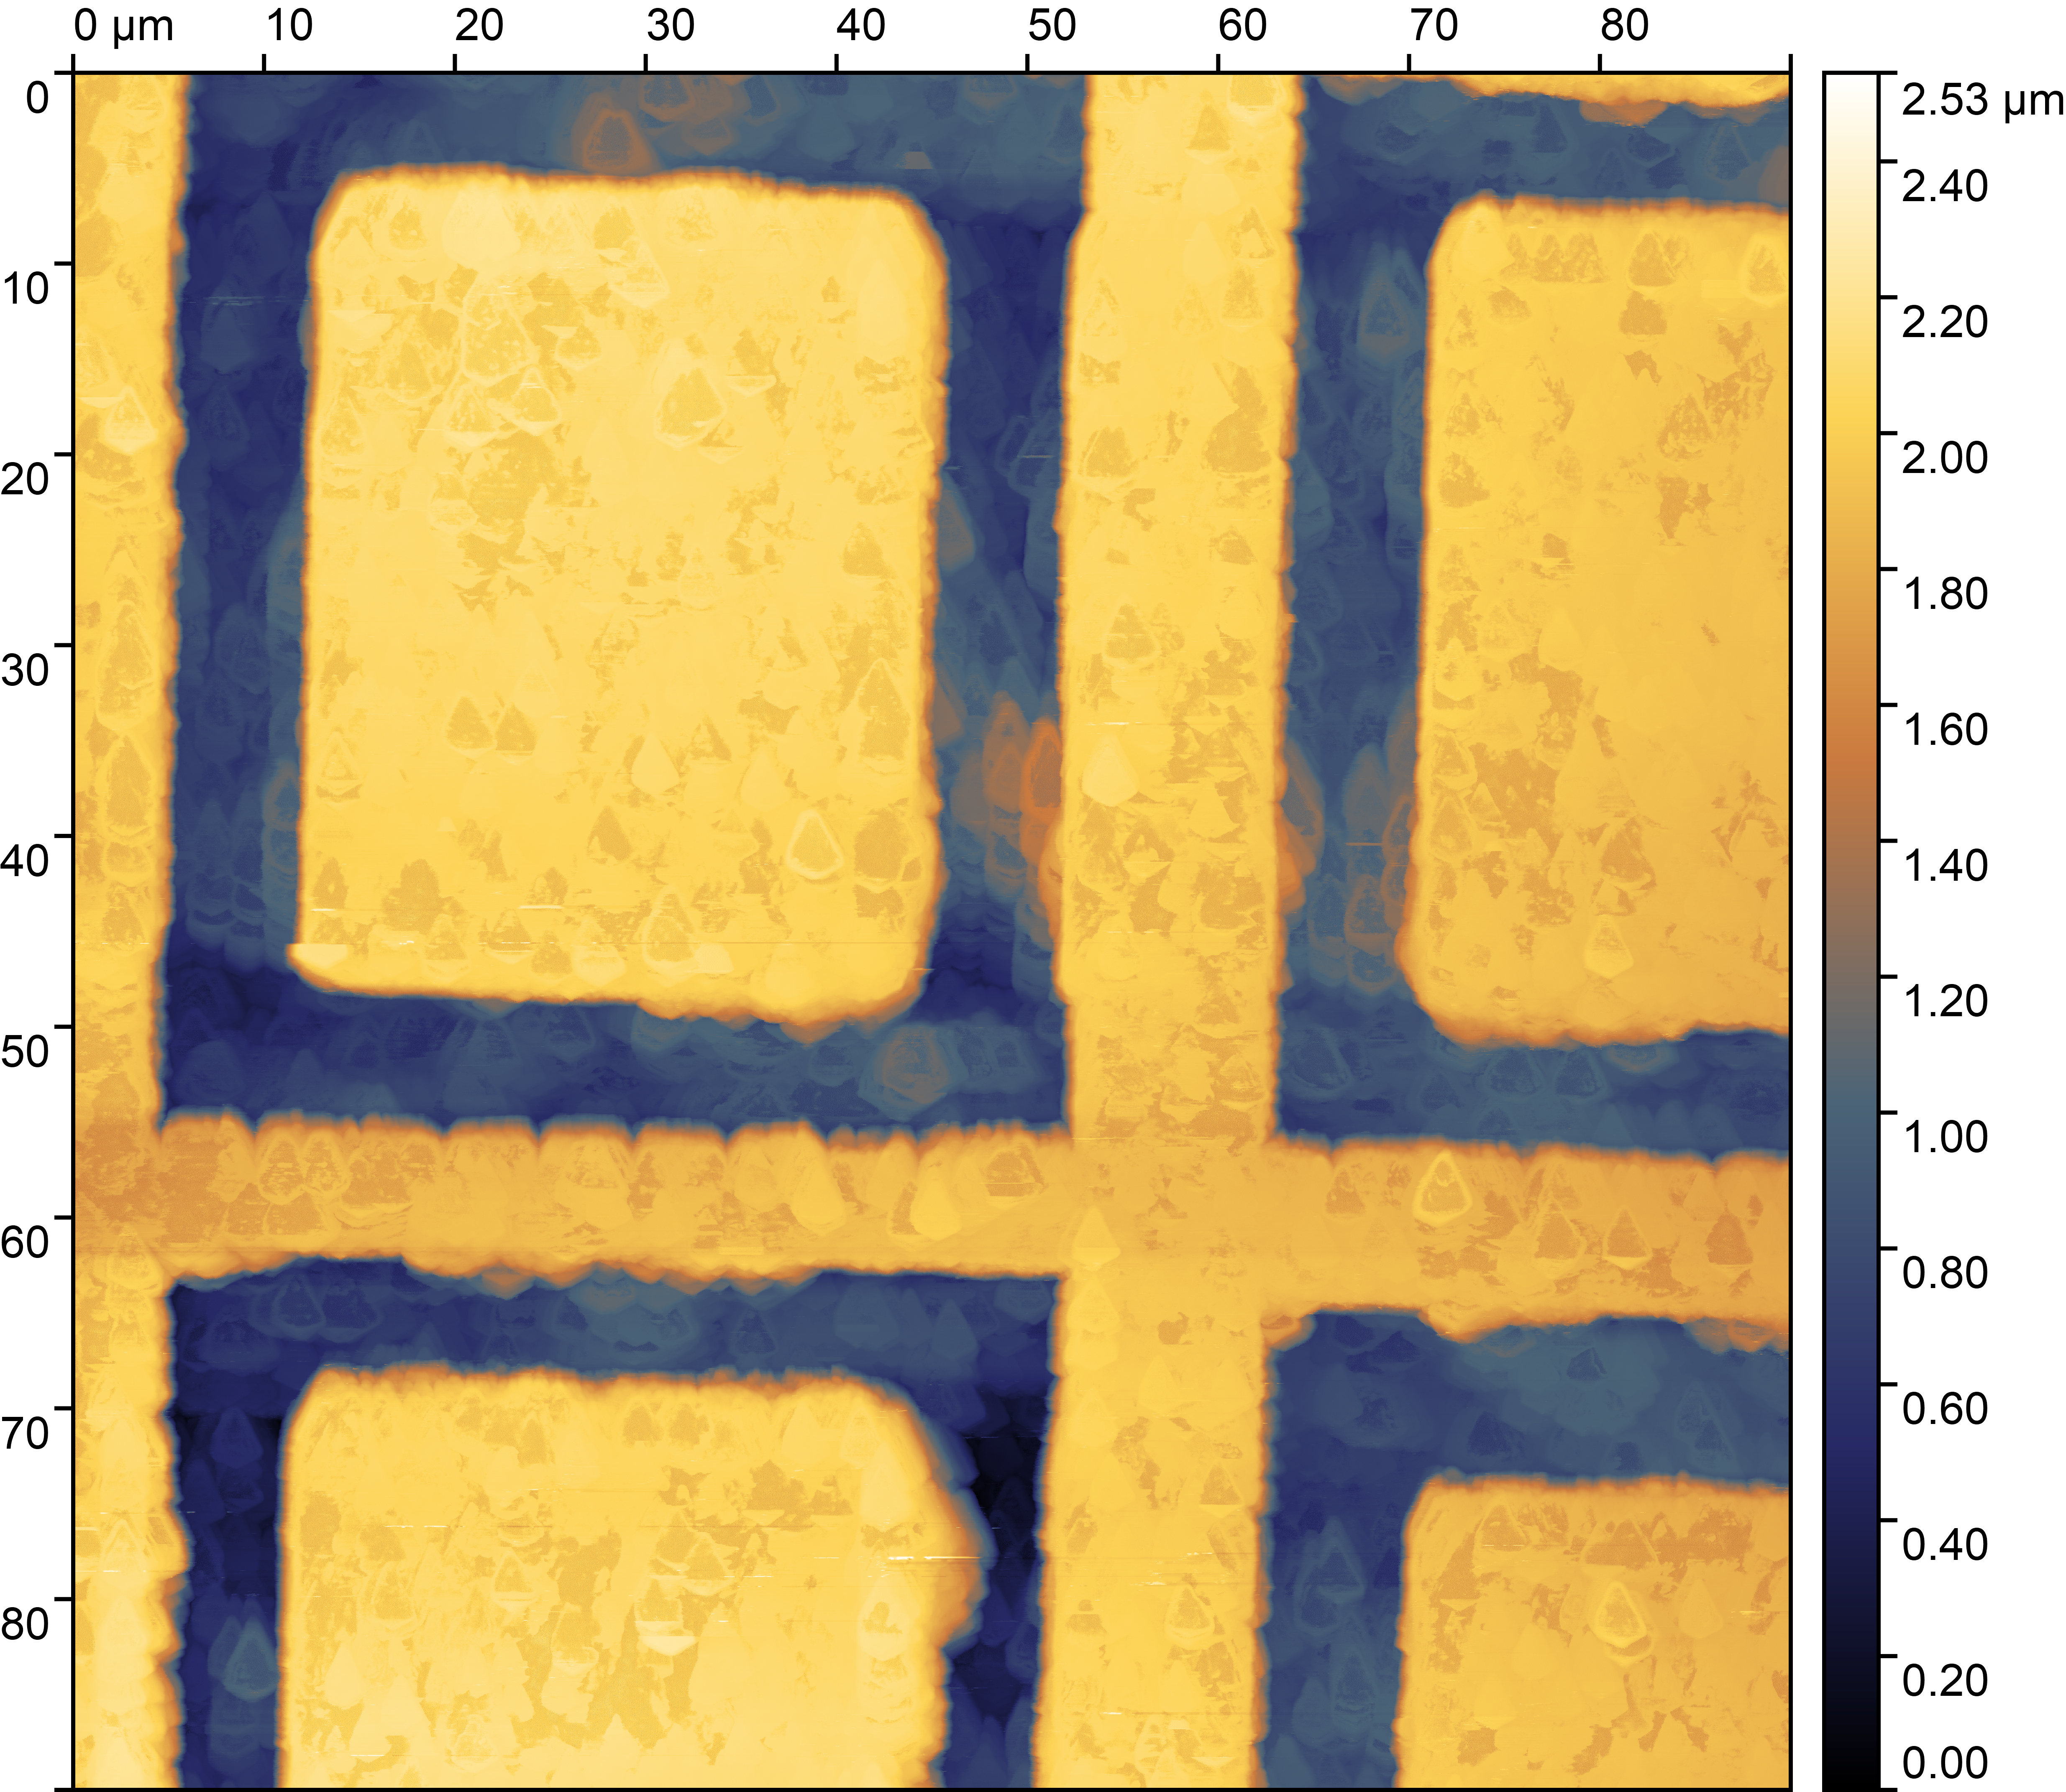
\includegraphics[width=\textwidth]{Chapter7/Figs/Raster/AF emitter array afm.jpg}
    \caption{A large area AFM scan of emitter array AF that was used for electrical characterisation.}
    \label{fig:afm_af_large}
\end{figure}

Figure \ref{fig:afm_af_large} shows a large area AFM scan that was taken to examine the effective topology of an emitter array type structure as written via laser graphitisation. In this figure, almost the entirety of contact A (top left) is visible, with contact F directly below (bottom left). In-between these two contacts, extending downwards from contact A, the beginnings of the laser written wire structures are just about visible as depressions in the topology. This also provides another general view of the laser writing process and the sometimes inconsistent structures that are written on the diamond surface. In some places, there are very noticeable protrusions from the sidewalls into the otherwise rectangular etched contact structures. As this is purely a topological scan, this hence displays a lack of ablation in these regions, perhaps due to a lack of graphitisation processes, lower laser absorption, or other changes in the writing process. Similarly, some areas within the contact structures appear to have a greater depth than the majority of written area, perhaps due to a greater absorption of laser power in these specific regions, or perhaps more readily graphitised and subsequently ablated diamond.

\begin{figure}[H]
    \centering
    \includegraphics[width=\textwidth]{Chapter7/Figs/Raster/af_cropped_emitters.jpg}
    \caption{A cropped AFM scan of emitter array AF that was used for electrical characterisation.}
    \label{fig:afm_af_crop}
\end{figure}

\begin{figure}[H]
    \centering
    \includegraphics[width=0.95\textwidth]{Chapter7/Figs/Raster/af_emitter_design1.png}
    \caption{A cropped view of the AF emitter array design, with feature size measurements provided.}
    \label{fig:afm_af_design}
\end{figure}

For clarity, the region between contacts A (upper) and F (lower) is cropped down and expanded in figure \ref{fig:afm_af_crop}. When compared directly with the designed array in figure \ref{fig:afm_af_design}, the topology does not directly reveal the presence of 0.8~\si{\micro\metre} width emitter wires extending down towards contact F. However, it is possible to see what may be the very start of all but the two outer emitter wires, with notable triangular depressions extending nearly as deep as the larger width contact structures.

\begin{figure}[H]
    \centering
    \includegraphics[width=\textwidth]{Chapter7/Figs/Raster/CH_cropped.jpg}
    \caption{A cropped AFM scan of the CH emitter array, with scan direction parallel to the emitter wires (y-axis).}
    \label{fig:afm_ch_array}
\end{figure}

Figure \ref{fig:afm_ch_array} shows another of the emitter array structures that were fabricated on the diamond surface. In contrast to the unclear topology observed with array AF, array CH appears to clearly demonstrate the presence of ablated diamond, and hence the fabrication of emitter wires leading down from contact C into the channel towards contact H. As observed in the wider AFM scans, the intended rectangular contact design for contact H in particular displays some deformation, with notable incongruities along the top of the graphitised region. The success of this AFM scan in displaying topographical results may be attributed to the y-axis scan direction, which is the fast direction. Based on the general observation from scan rate testing that higher scan rates will tend to show a lower slope of descent, and a higher angle of ascent, one clear practical approach to accurately detecting sub-micron thickness graphitised wires is to scan along the length of the emitter, rather than across the width. This ensures that the tip does not need to descend into the emitter channel, and instead as it passes down from the contact region, it will tend to only require a raised elevation as it progresses. When running in the reverse direction (up from contact H), again only one clear descent is necessary to enter the emitter channel, where the tip then remains as it passes down the channel. Hence, the slow scan rate direction is then across the width of the emitters, and is best able to detect any change in topology. A further detail with this approach is that this requires a suitable pixel density, as the number of pixels across the width of the emitter channel directly translates to the number of points along the length of the emitter where the tip will travel, measuring the depth of ablated material. Hence, in this example with a fast scan rate of 7.5~\si{\micro\metre\per\second} and a raw scan size of 62~\si{\micro\metre} x 15~\si{\micro\metre}, to observe emitter widths of 0.8~\si{\micro\metre}, the effective pixel width must be below 0.4~\si{\micro\metre} to ensure that the AFM tip does indeed enter the graphitised emitter channel, in a near central location. For this scan a pixel width of $\sim0.24$~\si{\micro\metre} appears to have been sufficient to positively identify ablation related to the formation of graphitised emitters, especially combined with the slow scan rate direction and the top-down AFM tip pass scan direction.

The design of emitter array CH was otherwise very similar to AF, with 10 emitter cathodes of width 0.8~\si{\micro\metre} spaced 4.2~\si{\micro\metre} apart across the 60~\si{\micro\metre} contact structure (C). The only difference was in the cathode-anode spacing, due to a slight shortening of the emitter wire, which in the case of AF was 2~\si{\micro\metre}, and for CH was 2.5~\si{\micro\metre}. Preliminary low resolution AFM scans indicated that array CH was one of the clearest examples of the intended emitter structure, and so this was selected for electrical characterisation alongside AF.

\subsection{Fluorescence Characterisation}
\label{subsec:fluorescence_characterisation}

\begin{figure}[H]
    \centering
    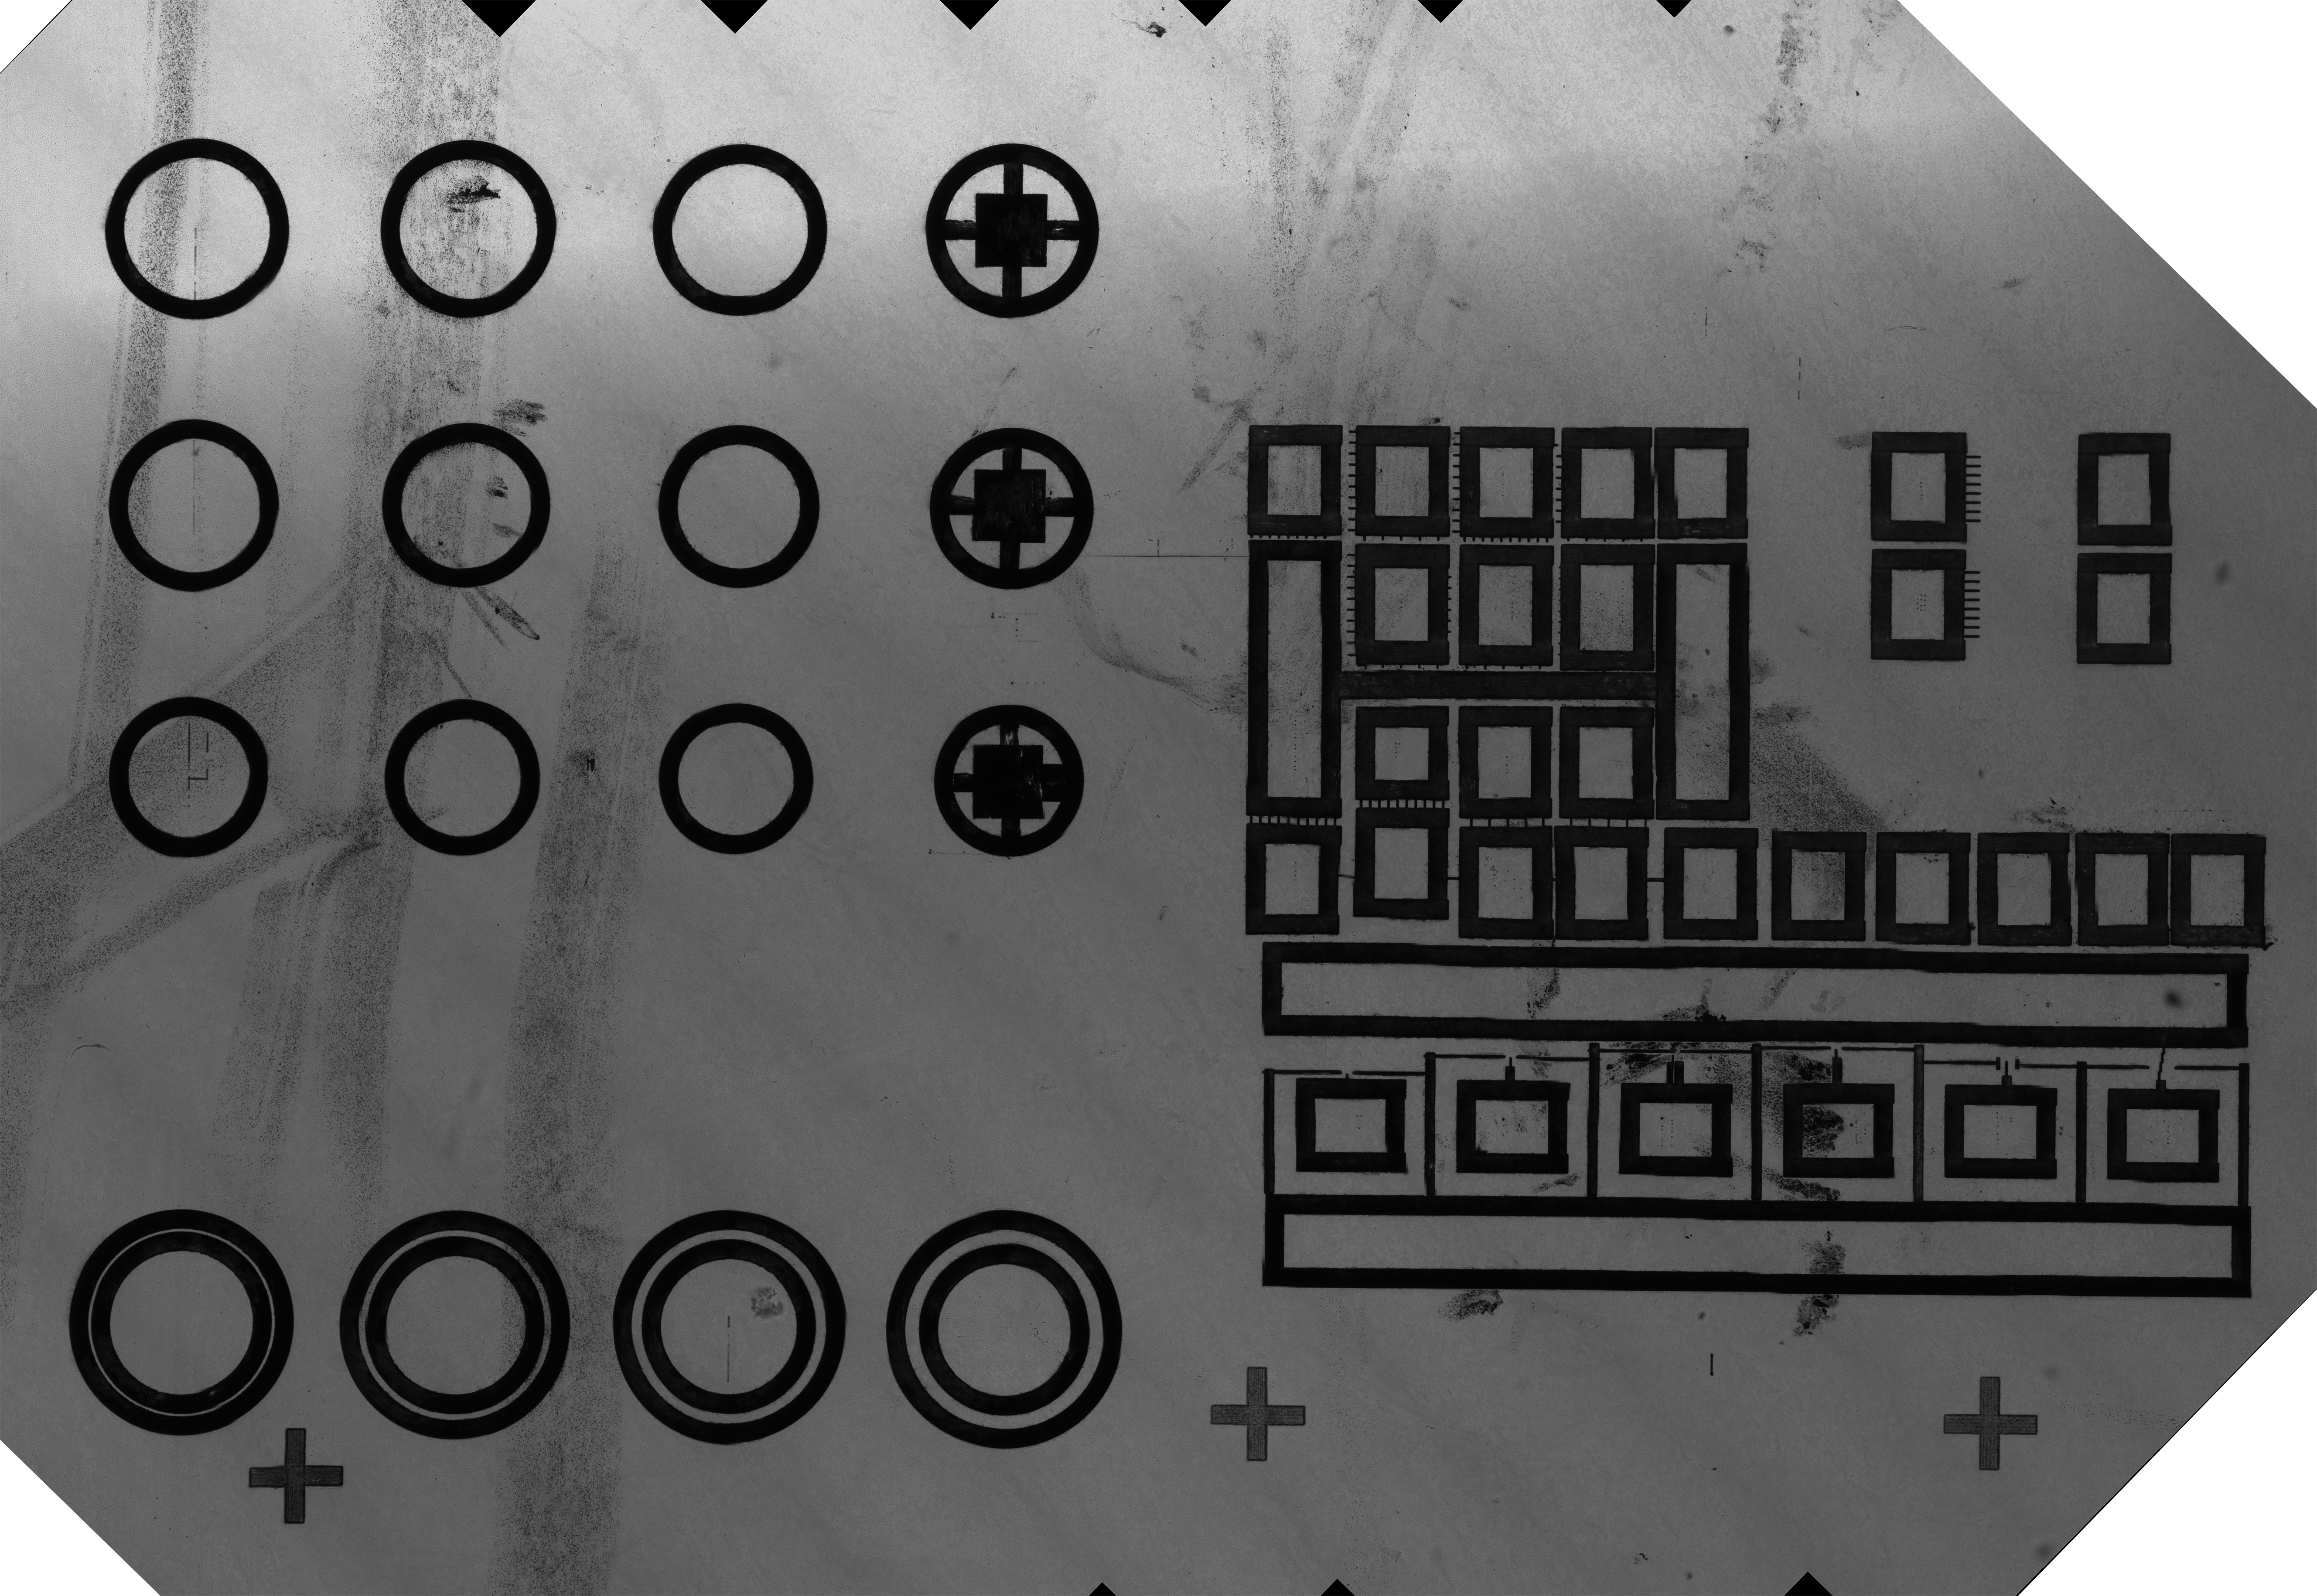
\includegraphics[width=\textwidth]{Chapter7/Figs/Raster/ESID_rotated_downscaled_further.jpg}
    \caption{An overview of the laser graphitised structure as seen using a backlit 488~\si{\nano\metre} light source and mapping with a confocal microscope.}
    \label{fig:bio_esid}
\end{figure}

One possible source of material characterisation is that of fluorescence. Figure \ref{fig:bio_esid} shows the optical overview provided by the Zeiss LSM 800 system, providing a grouped map of confocal scans that allows for near-diffraction-limited imaging across the entirety of the laser-written structures. The images provided by this system allow for good optical comparisons with the topological AFM measurements, with the change in observed 488~\si{\nano\metre} absorbance due to the graphitisation or amorphisation of carbon perhaps providing a more reliable picture of how well the fabrication of the thinnest laser treated features have formed. Further to this, diamond fluorescence centres offer a unique examination of the composition of diamond defects. In particular, it should be expected that HPHT samples such as those used for the substrates in the current work will have a large concentration of singly substitutional nitrogen, aka C-centres. This imparts the deep yellow-orange colour as is typical for HPHT samples when seen by the naked eye, and is a substantial factor in the characteristic fluorescence of HPHT grown diamonds. 

\begin{figure}[H]
    \centering
    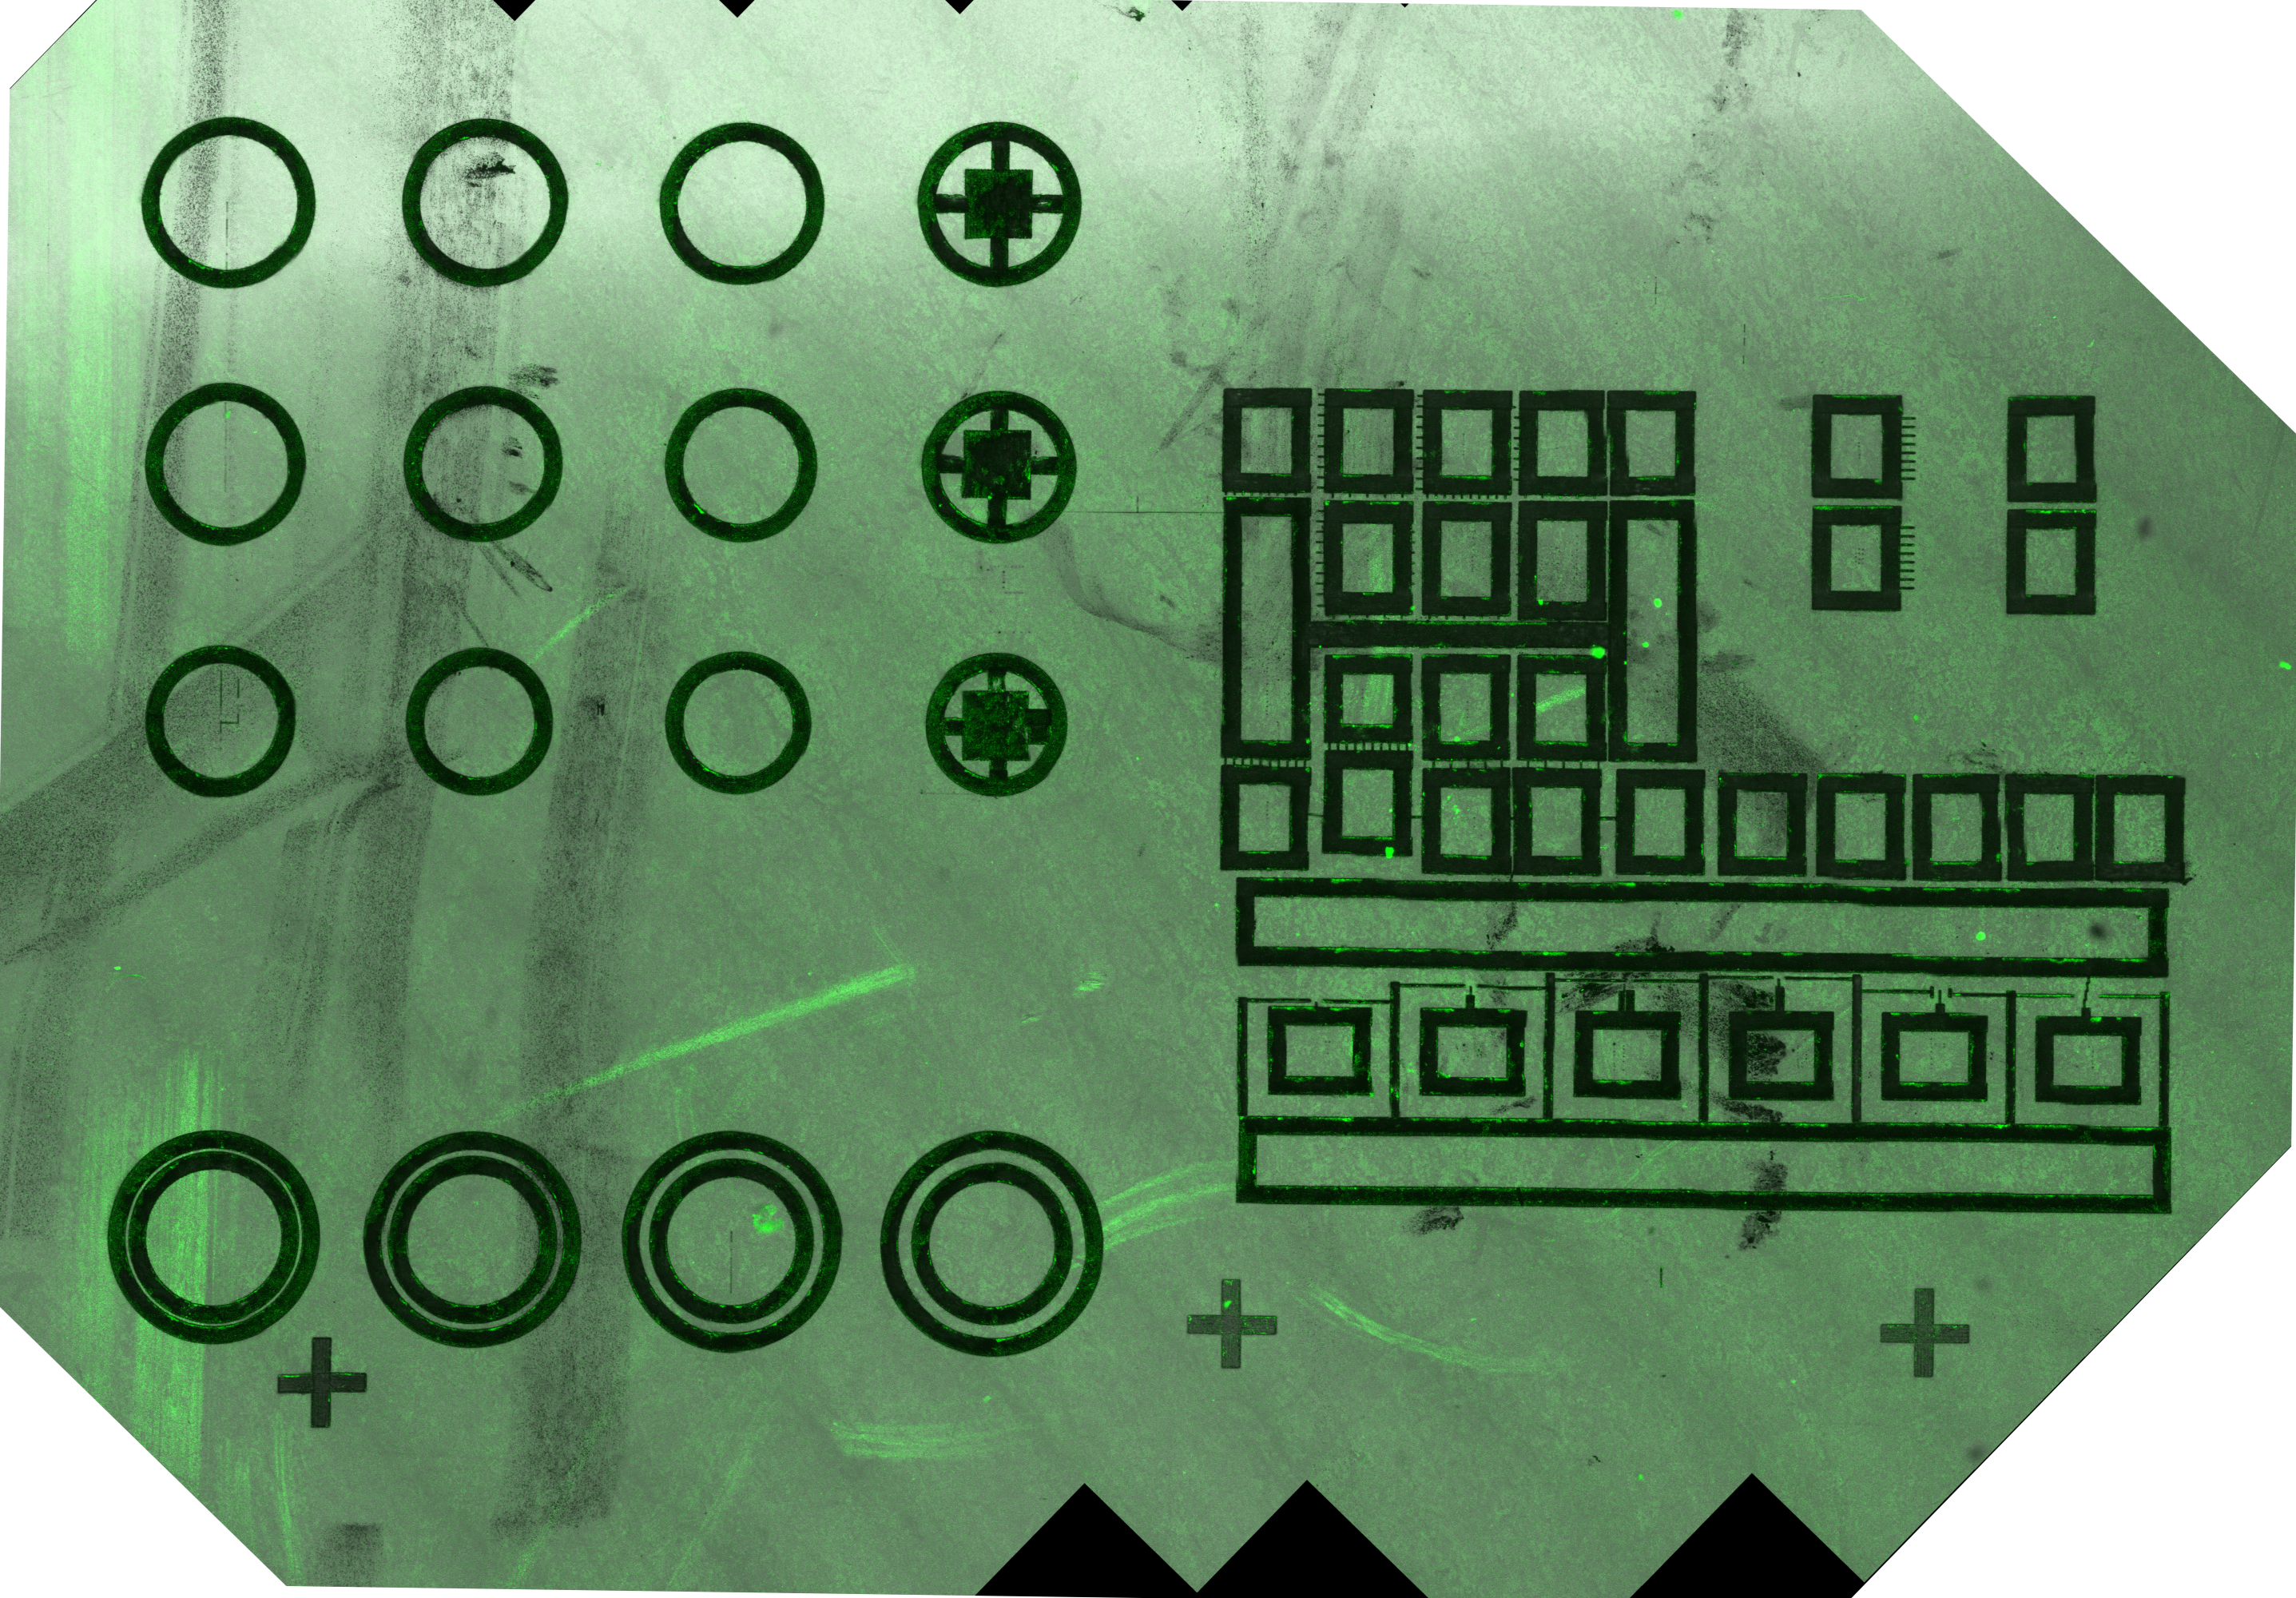
\includegraphics[width=\textwidth]{Chapter7/Figs/Raster/FL_overview.jpg}
    \caption{A confocal microscope mapping overview of the laser written structures as seen using a backlit 488~\si{\nano\metre} light source. The green false colour is provided by fluorescence using an excitation laser of 408~\si{\nano\metre}.}
    \label{fig:fl_overview}
\end{figure}

Figure \ref{fig:fl_overview} shows the overlay of a false colour (green) fluorescence scan with excitation laser 408~\si{\nano\metre} onto the original 488~\si{\nano\metre} absorption imaging from figure \ref{fig:bio_esid}. A few observations can be made regarding this experiment, beginning with the clear background fluorescence throughout the sample. This is due to the substrate itself, as is expected for a typical HPHT sample \cite{eaton2017, zhao2023}. However, while the background fluorescence has a reasonably steady profile, there are significant deviations visible. 

\subsubsection{Source of Fluorescence}
\label{subsubsec:source_of_fluorescence}
During the setup of the fluorescence imaging shown in this section, a sweep of the fluorescence emission spectrum was performed by utilising the range of colour filters available in the Zeiss LSM 800 system. The available colour filters thus provided an estimate of the wavelength of fluorescence emission within 20~\si{\nano\metre} ranges, and showed that the most significant wavelength detection was within the 500--520~\si{\nano\metre} range. The exact defects responsible for the fluorescence that is concentrated on the laser processed portions cannot be determined precisely with the collected data presented here. The exact defect emission wavelengths can differ due to temperature differences, crystal strain and excitation wavelength, making exact identification difficult even under ideal circumstances \cite{Jones2020} though more recent applications of machine learning statistical methods allow for much lower error rates \cite{Hardman2022}. 

Despite the challenge in defect identification, one possibility that must be considered for the observed regions of intense fluorescence at the edges of laser processing is that of etching through the phosphorous doped surface layer to allow for more light emission from the substrate underneath. This is unlikely, as the AFM appears to show an inverse correlation with the fluorescent laser processed diamond and the height. That is to say that the regions which display discolouration (darkening) and hence an increased concentration of amorphous carbon without deep etching through the phosphorous doped layer also appear to have fluorescent regions in certain locations.

The incorporation of nitrogen into the HPHT grown substrate in the absence of a nitrogen getter is largely dependent upon growth facets, with the growth sectors \hkl{111} containing the highest concentrations of nitrogen \cite{kanda2000}. This leads to a clear pattern of colour corresponding to a change in optically active defects, with the sample used for laser graphitisation in this case being no exception to this growth process. A notable observation from figure \ref{fig:fl_overview} was that of a relatively uniform background fluorescence, alongside the non-uniform, concentrated fluorescence of the laser processed devices. This also implies that the larger concentration of C centres leading to visible colouration of growth facets has not altered the concentration or distribution of fluorescing colour centres within the diamond, though the possibility of fluorescence being due to organic molecules etc cannot be excluded entirely based on this analysis alone. 

\begin{table}[h]
\centering
\begin{tabular}{|l|l|l|l|}
\hline
\textbf{Defect Type} & \textbf{Excitation (nm)} & \textbf{Fluorescence (nm)} \\
\hline
N3V & 365 (LW) & 415,  440 (1) \\
H3 (NVN$^{0}$) & 365 (LW) & 503, 530 (1), 510 (3,4) \\
H4 (N$_{4}$V$_{2}$) & 365 (LW) & 496, 520 (1,3) \\
480 nm band & 365 (LW), varies & 480, varies (1), $\sim$540 (3) \\
NV\textsuperscript{0} & 532 & 575 (ZPL) (1,2) \\
NV\textsuperscript{-} & 532 & 637 (ZPL) (1,2) \\
Unknown & Not specified & 370-380 (Newly observed) (2) \\
3H Split interstitial $\langle100\rangle$ & Not specified & 504--510, 532 (Paired bands) (2,5) \\
\hline
\end{tabular}

\caption{Overview of defects in HPHT diamonds, excitation wavelengths (long wave LW, short wave SW), and specific fluorescence wavelengths as discussed in (1) \cite{eaton2017}, (2) \cite{burachenko2021}, (3) \cite{shigley2013}, (4) \cite{shenderova2019}, (5) \cite{Hardman2022}.}
\label{tab:fl_defects}
\end{table}

Table \ref{tab:fl_defects} provides a general overview of defects observed in diamond fluorescence spectroscopy. This represents only a small sub-sample of the many identified fluorescent defects and a couple of unidentified defects to help illustrate the number of unknowns within this spectroscopic analysis. While effort has been made to associate the observed fluorescence wavelength with the excitation wavelength, this is a parameter which is less commonly reported in full, and so the usage of a 408~\si{\nano\metre} laser does complicate the direct comparison to literature values. Of particular note for HPHT samples is the general identification of fluorescence when exposed to SW-UV \cite{eaton2017, shigley2013}, in contrast to the LW dependent fluorescence of natural diamonds. Identification of the exact colour centres responsible for this fluorescence varies from sample to sample, however NV centres of various charge states are the most likely candidate for the HPHT samples used in this work. Additional defects which should not have appreciable concentrations are included to give a broader overview of diamond fluorescence, with the H3 aggregate in particular providing one potential colour centre in the range observed by the spectroscopic estimate provided with the Zeiss LSM 800 system. This is despite the expectation of a lack of nitrogen aggregation in typical \hkl(111) HPHT diamond due to the growth process itself \cite{Burns1999}. Another possibility is the unintentional introduction of NV colour centres via laser processing \cite{chen2016}, which may then be possible to see around laser processing for device manufacturing. 

\begin{figure}[H]
\centering
\begin{subfigure}[t]{0.47\textwidth}
    \includegraphics[width=\textwidth]{Chapter7/Figs/Raster/optical front light.jpg}
    \caption{Typical frontal white LED illumination.}
    \label{fig:G_front}
\end{subfigure}
\hfill
\begin{subfigure}[t]{0.47\textwidth}
    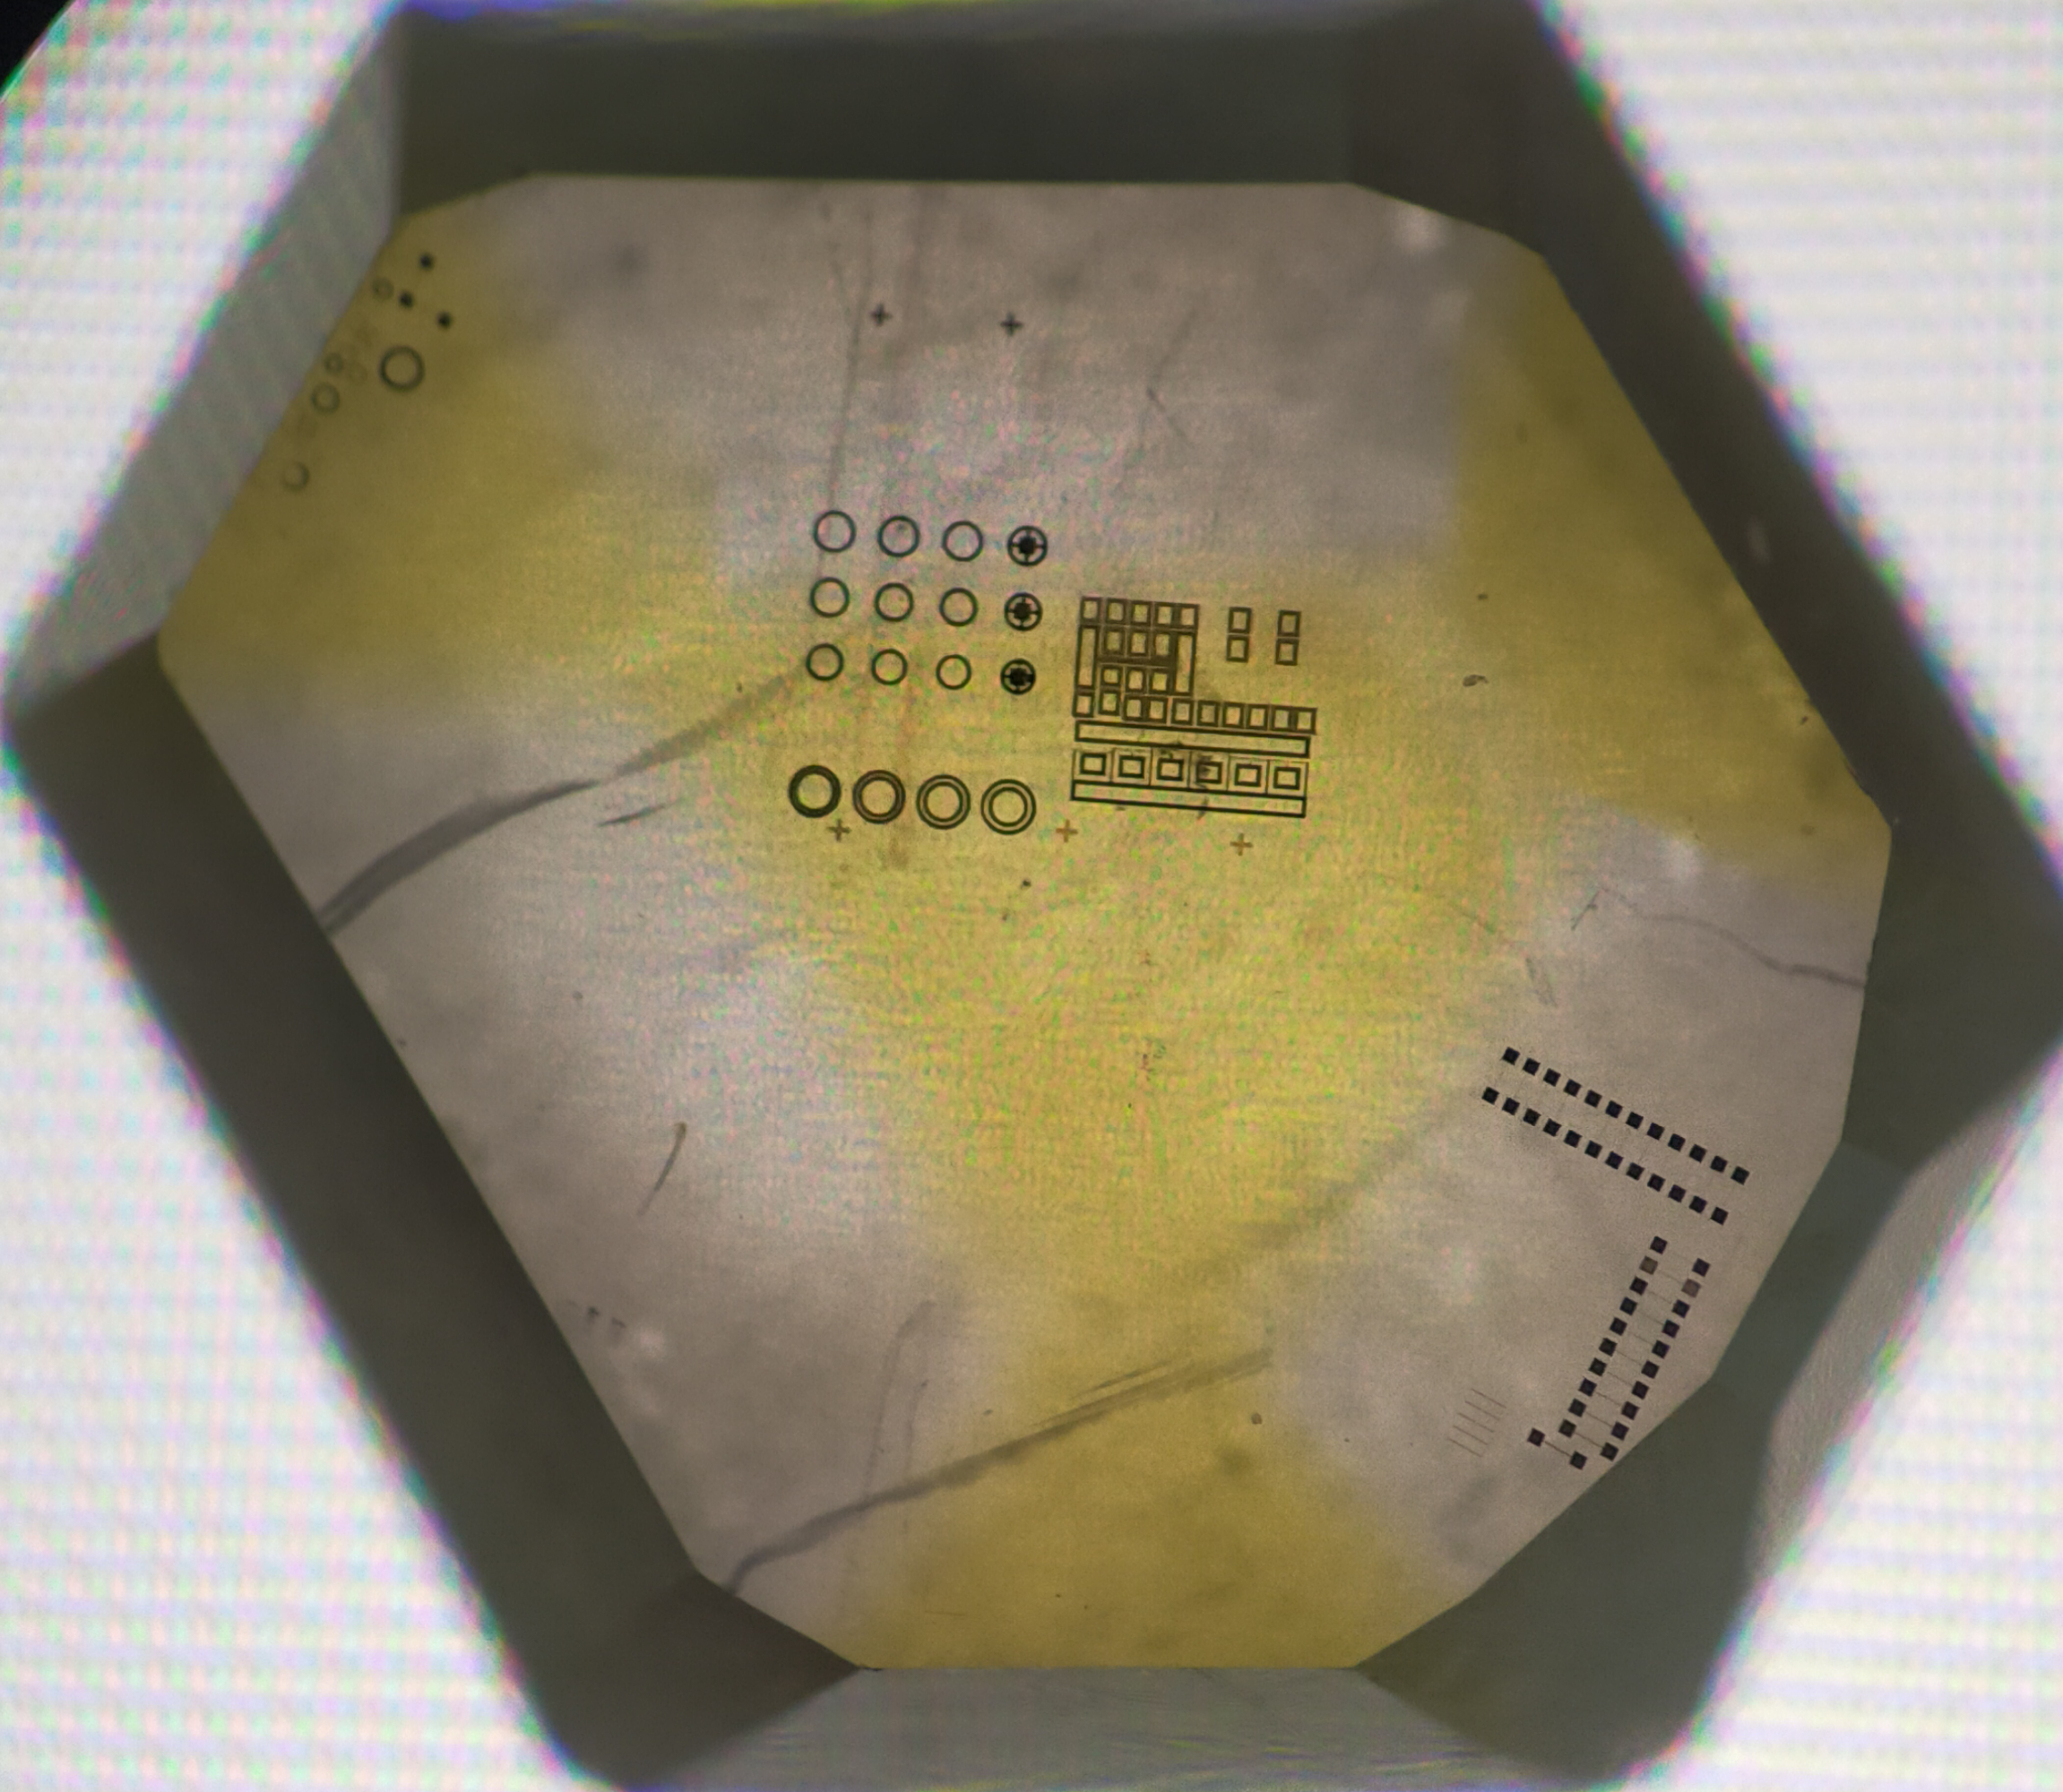
\includegraphics[width=\textwidth]{Chapter7/Figs/Raster/optical back light.jpg}
    \caption{Back-lighting provided by a RGB array.}
    \label{fig:G_back}
\end{subfigure}

\vspace{1em} % this will add some vertical space between the rows

\begin{subfigure}[t]{0.47\textwidth}
    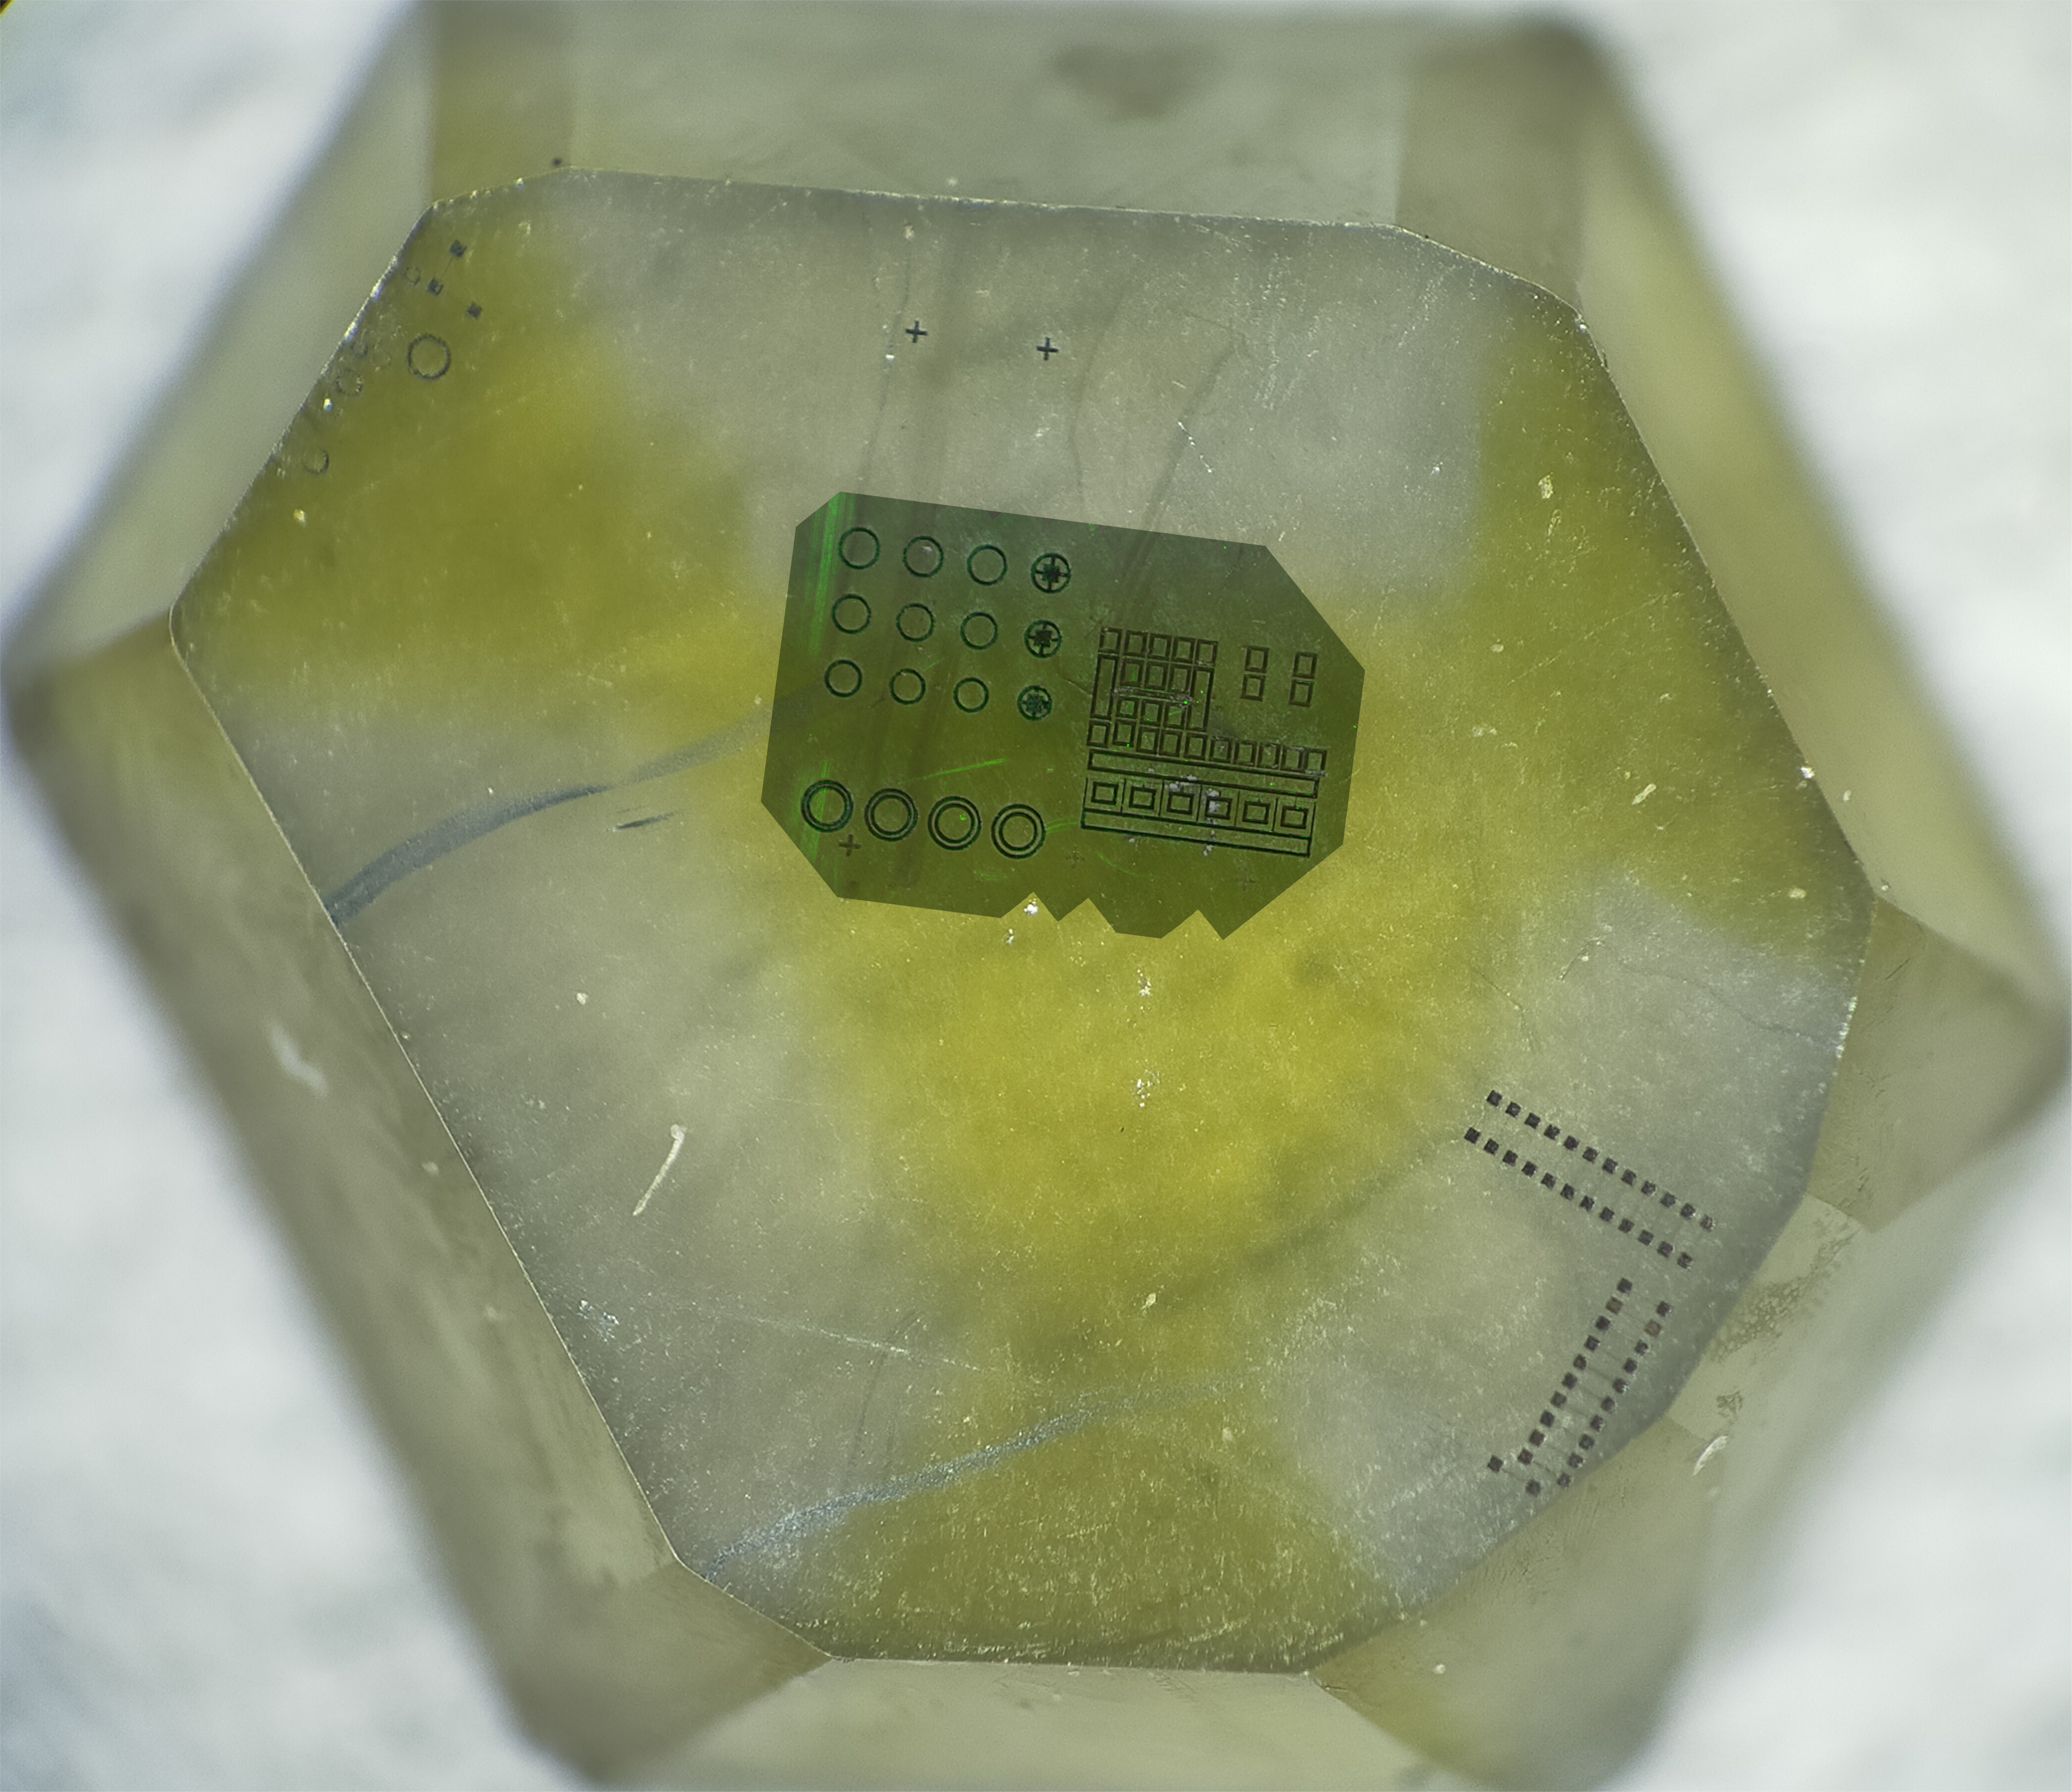
\includegraphics[width=\textwidth]{Chapter7/Figs/Raster/optical front light overlay.jpg}
    \caption{Frontal illumination and fluorescence overlay.}
    \label{fig:G_front_overlay}
\end{subfigure}
\hfill
\begin{subfigure}[t]{0.47\textwidth}
    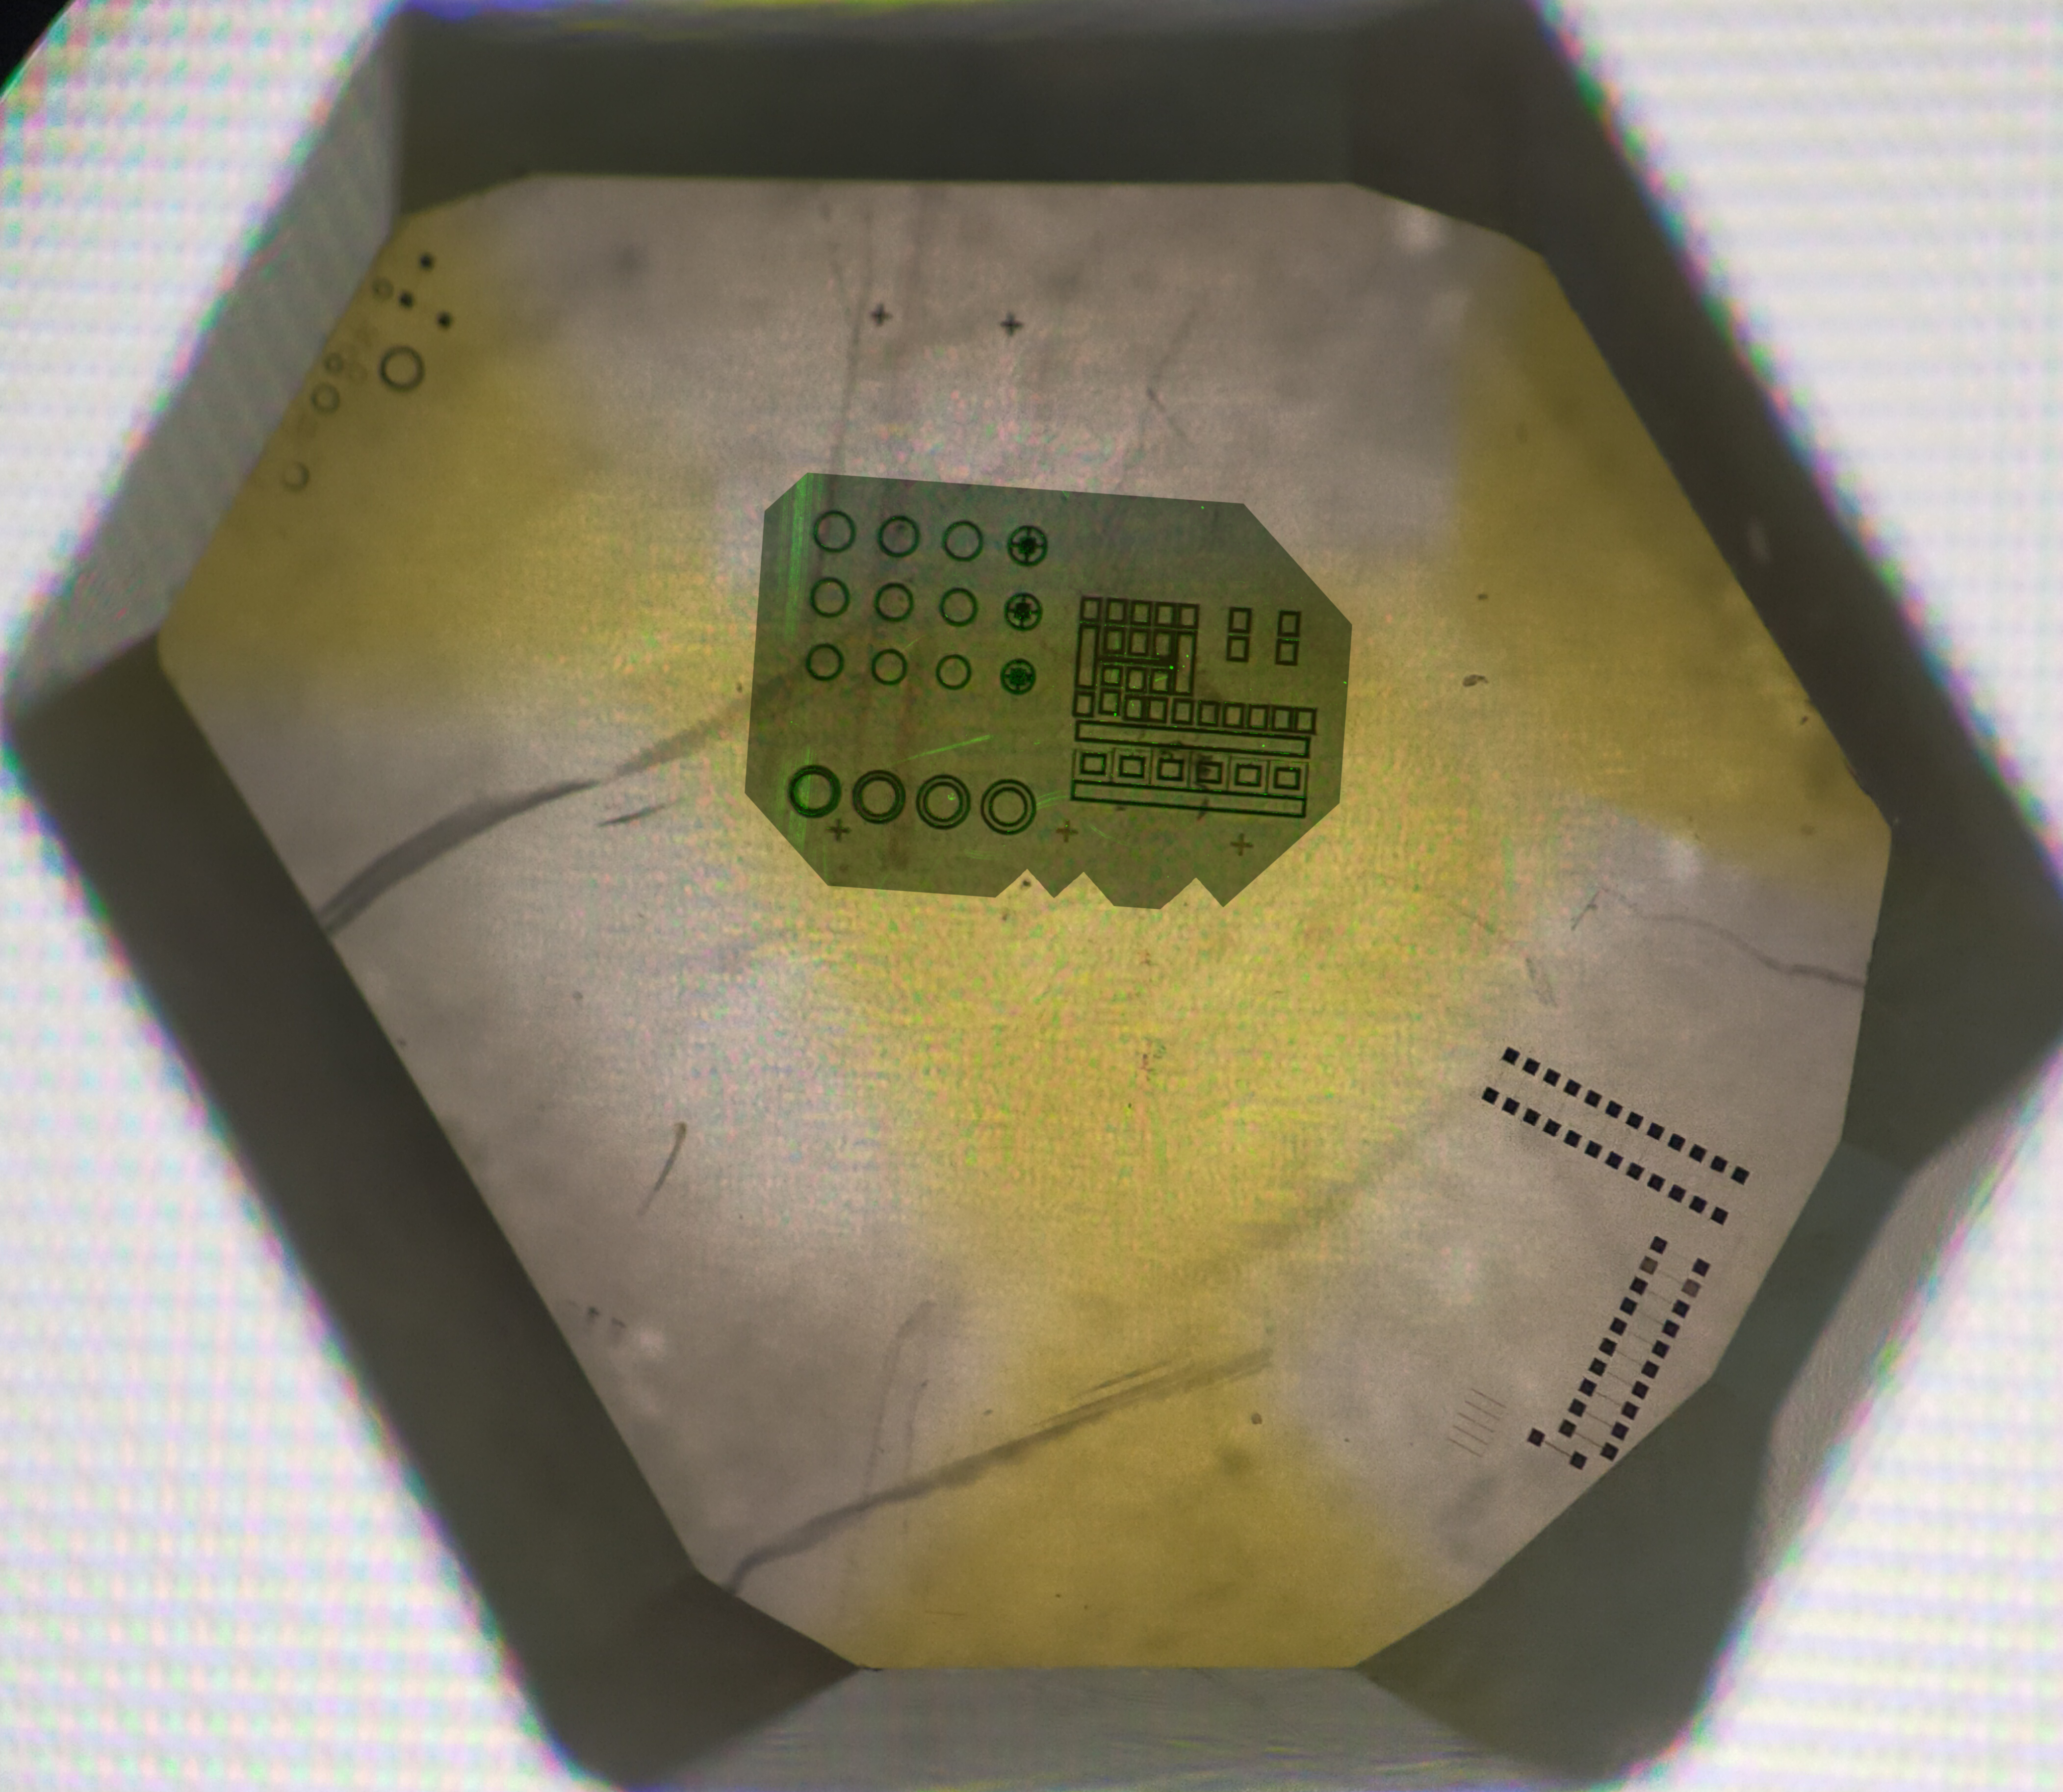
\includegraphics[width=\textwidth]{Chapter7/Figs/Raster/optical back light overlay.jpg}
    \caption{Back-lighting and fluorescence overlay.}
    \label{fig:G_back_overlay}
\end{subfigure}
\caption{Sample G as seen with a 3.6X magnification optical microscope, either direct front facing light or back-lighting, and the fluorescence imaging overlaid on these two images of differing lighting.}
\label{fig:G_illuminations}
\end{figure}

Figure \ref{fig:G_illuminations} includes two different approaches to taking optical images of the sample at a macroscopic scale, to demonstrate the visually apparent growth sectors within the HPHT sample. Back-lighting has a significant impact on the clarity and colour of the different growth sectors, as seen in figures \ref{fig:G_back}, \ref{fig:G_back_overlay}. In particular, a change in the substrate background colour can be observed near the top of the laser processed region, and it is possible to pick out the differing growth regions from the HPHT seed crystal.

\begin{figure}[H]
    \centering
    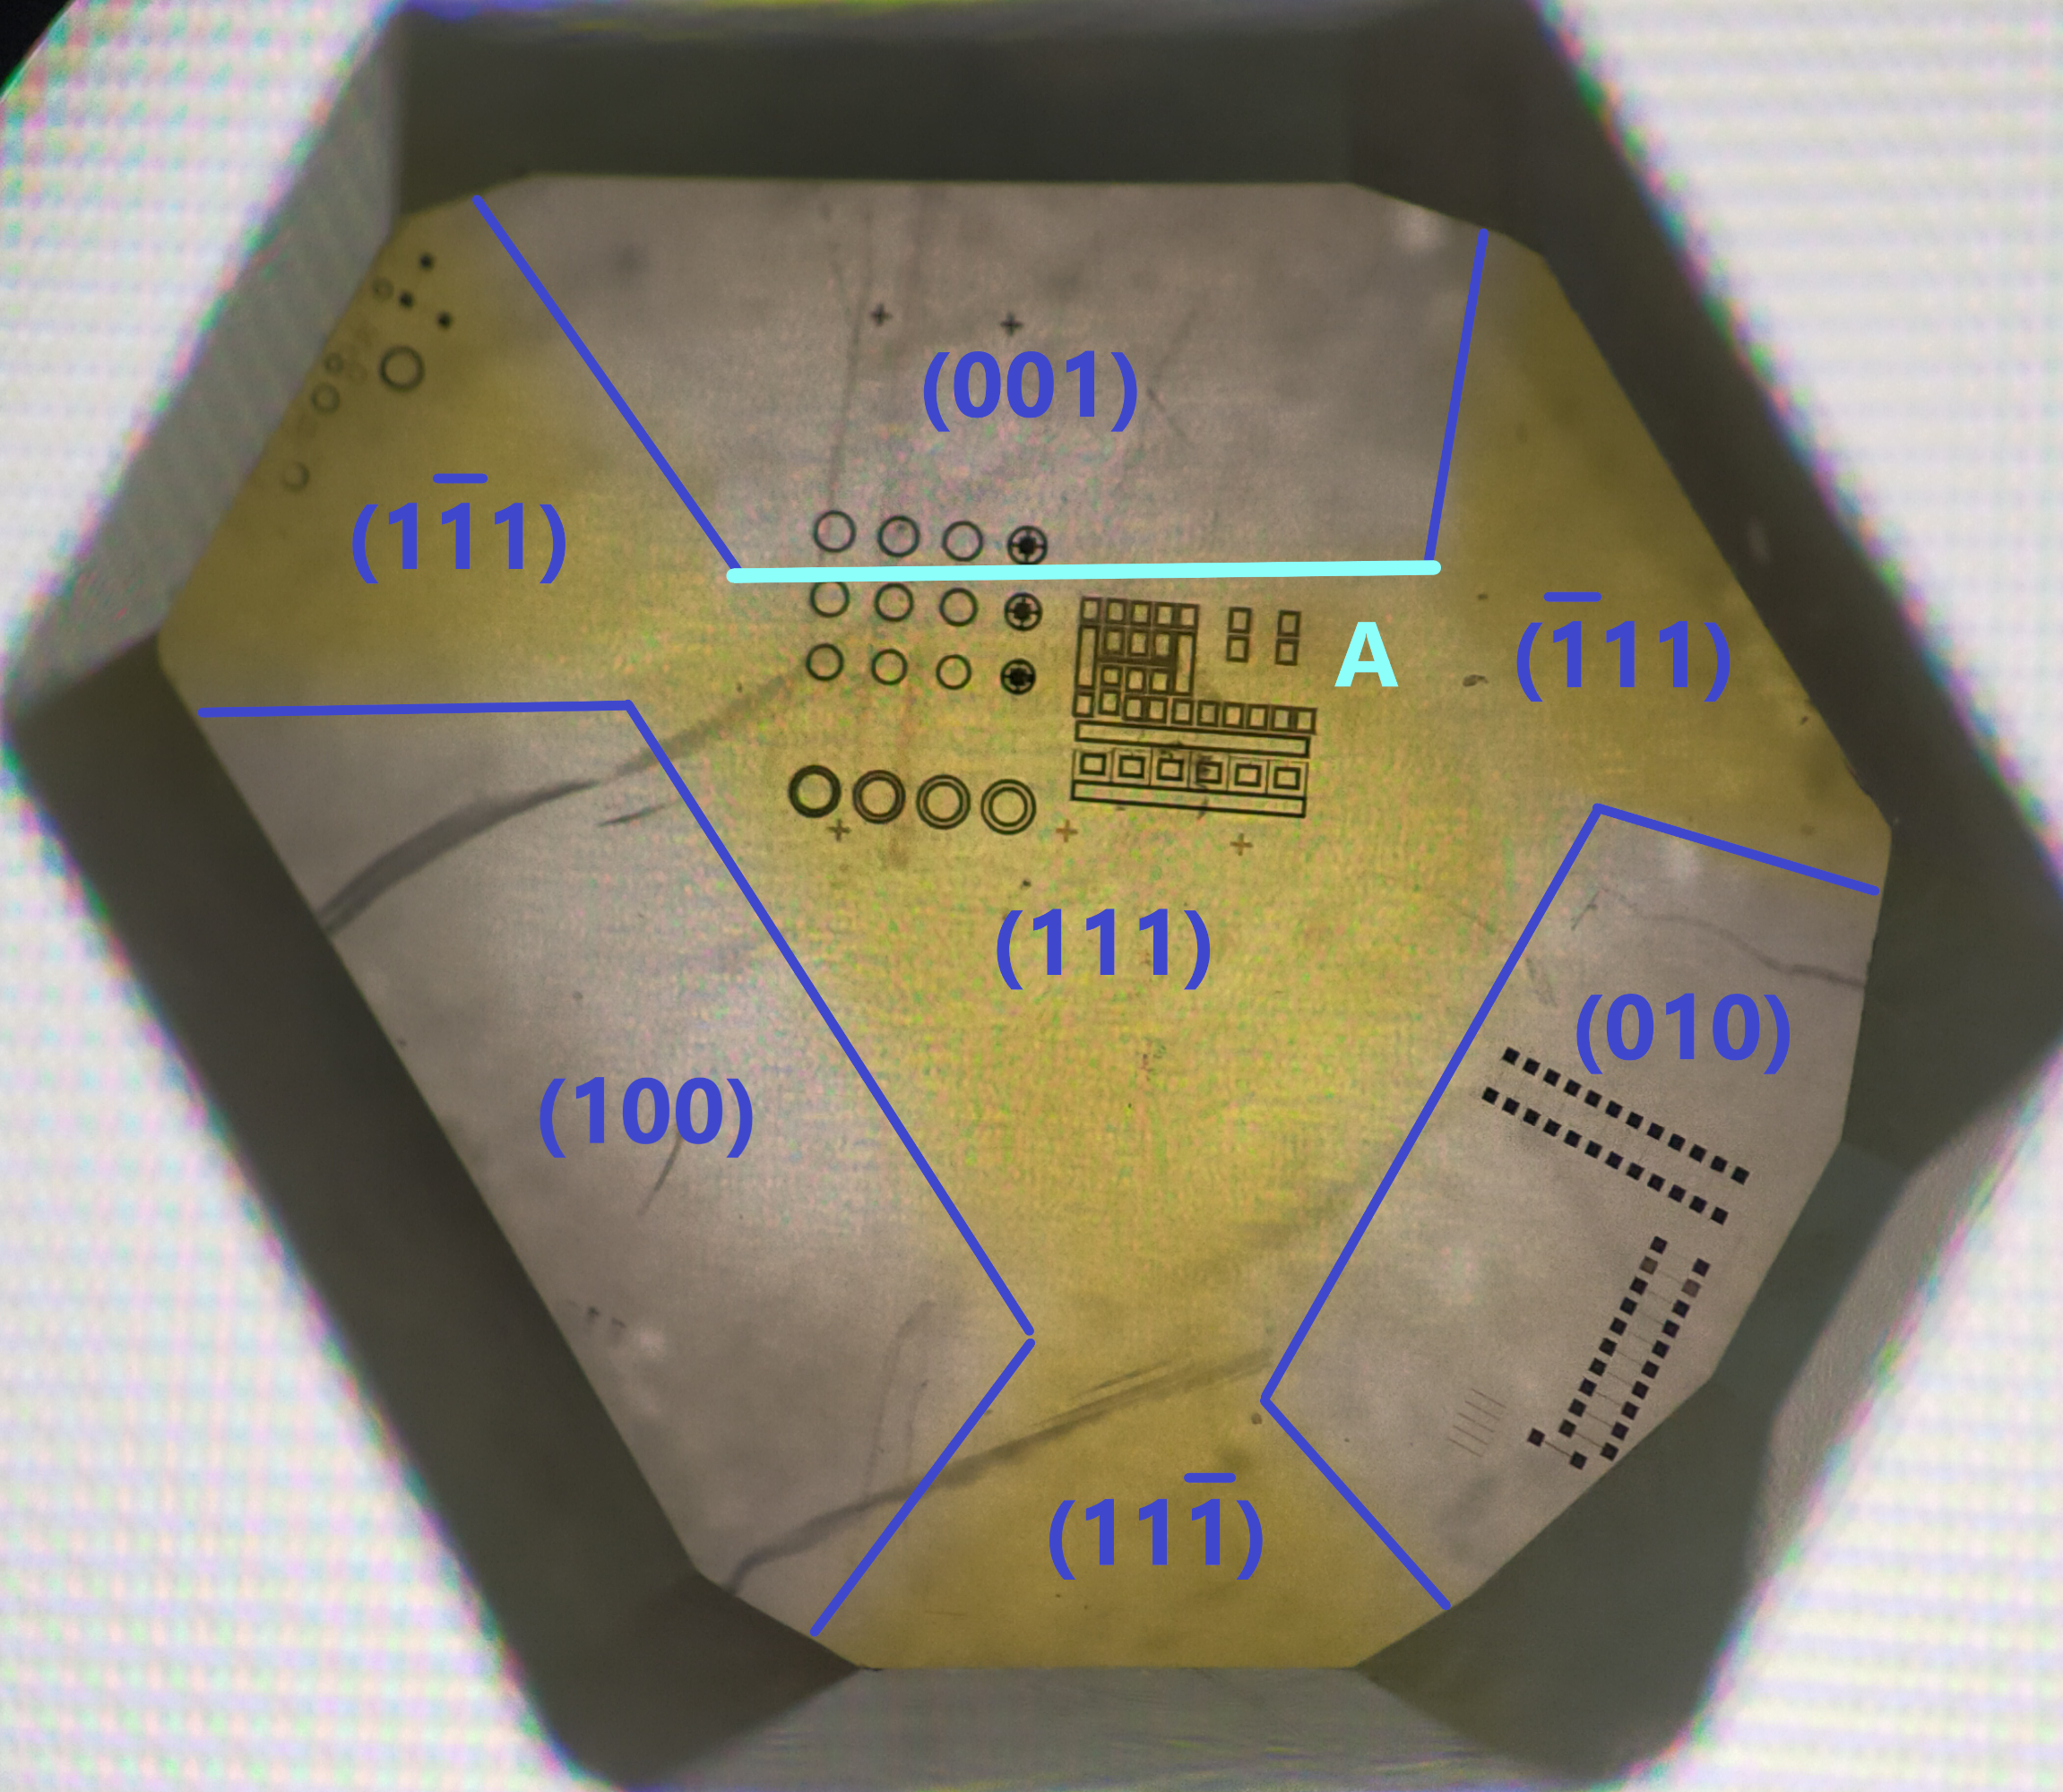
\includegraphics[width=0.8\linewidth]{Chapter7/Figs/Raster/48MP white 5 aperture graphite focus_crop_annotated 1_low.jpg}
    \caption{An annotated version of the back-lit optical microscope image to highlight growth sectors and the significant change in colouration running through the laser processed region.}
    \label{fig:G_annotated}
\end{figure}

Figure \ref{fig:G_annotated} provides an annotated form of figure \ref{fig:G_back}, to clarify the relevant growth sectors and also highlight the distinct change in colour centres that is observed across line A. Comparisons to the fluorescence reveal that the background fluorescence does not change significantly in density despite this change in absorbed/transmitted light.

\begin{figure}[H]
    \centering
    \includegraphics[width=0.8\linewidth]{Chapter7/Figs/Raster/FL_crop 3_low_annotated.jpg}
    \caption{A section of the fluorescence microscopy.}
    \label{fig:fl_crop3}
\end{figure}

In figure \ref{fig:fl_crop3}, the section around line A from figure \ref{fig:G_annotated} is presented to highlight the lack of background growth sector specificity in the observed, relatively constant background fluorescence. The estimated location of the optically observed growth sector change and subsequent change in nitrogen content is indicated by line A.

\begin{figure}[H]
    \centering
    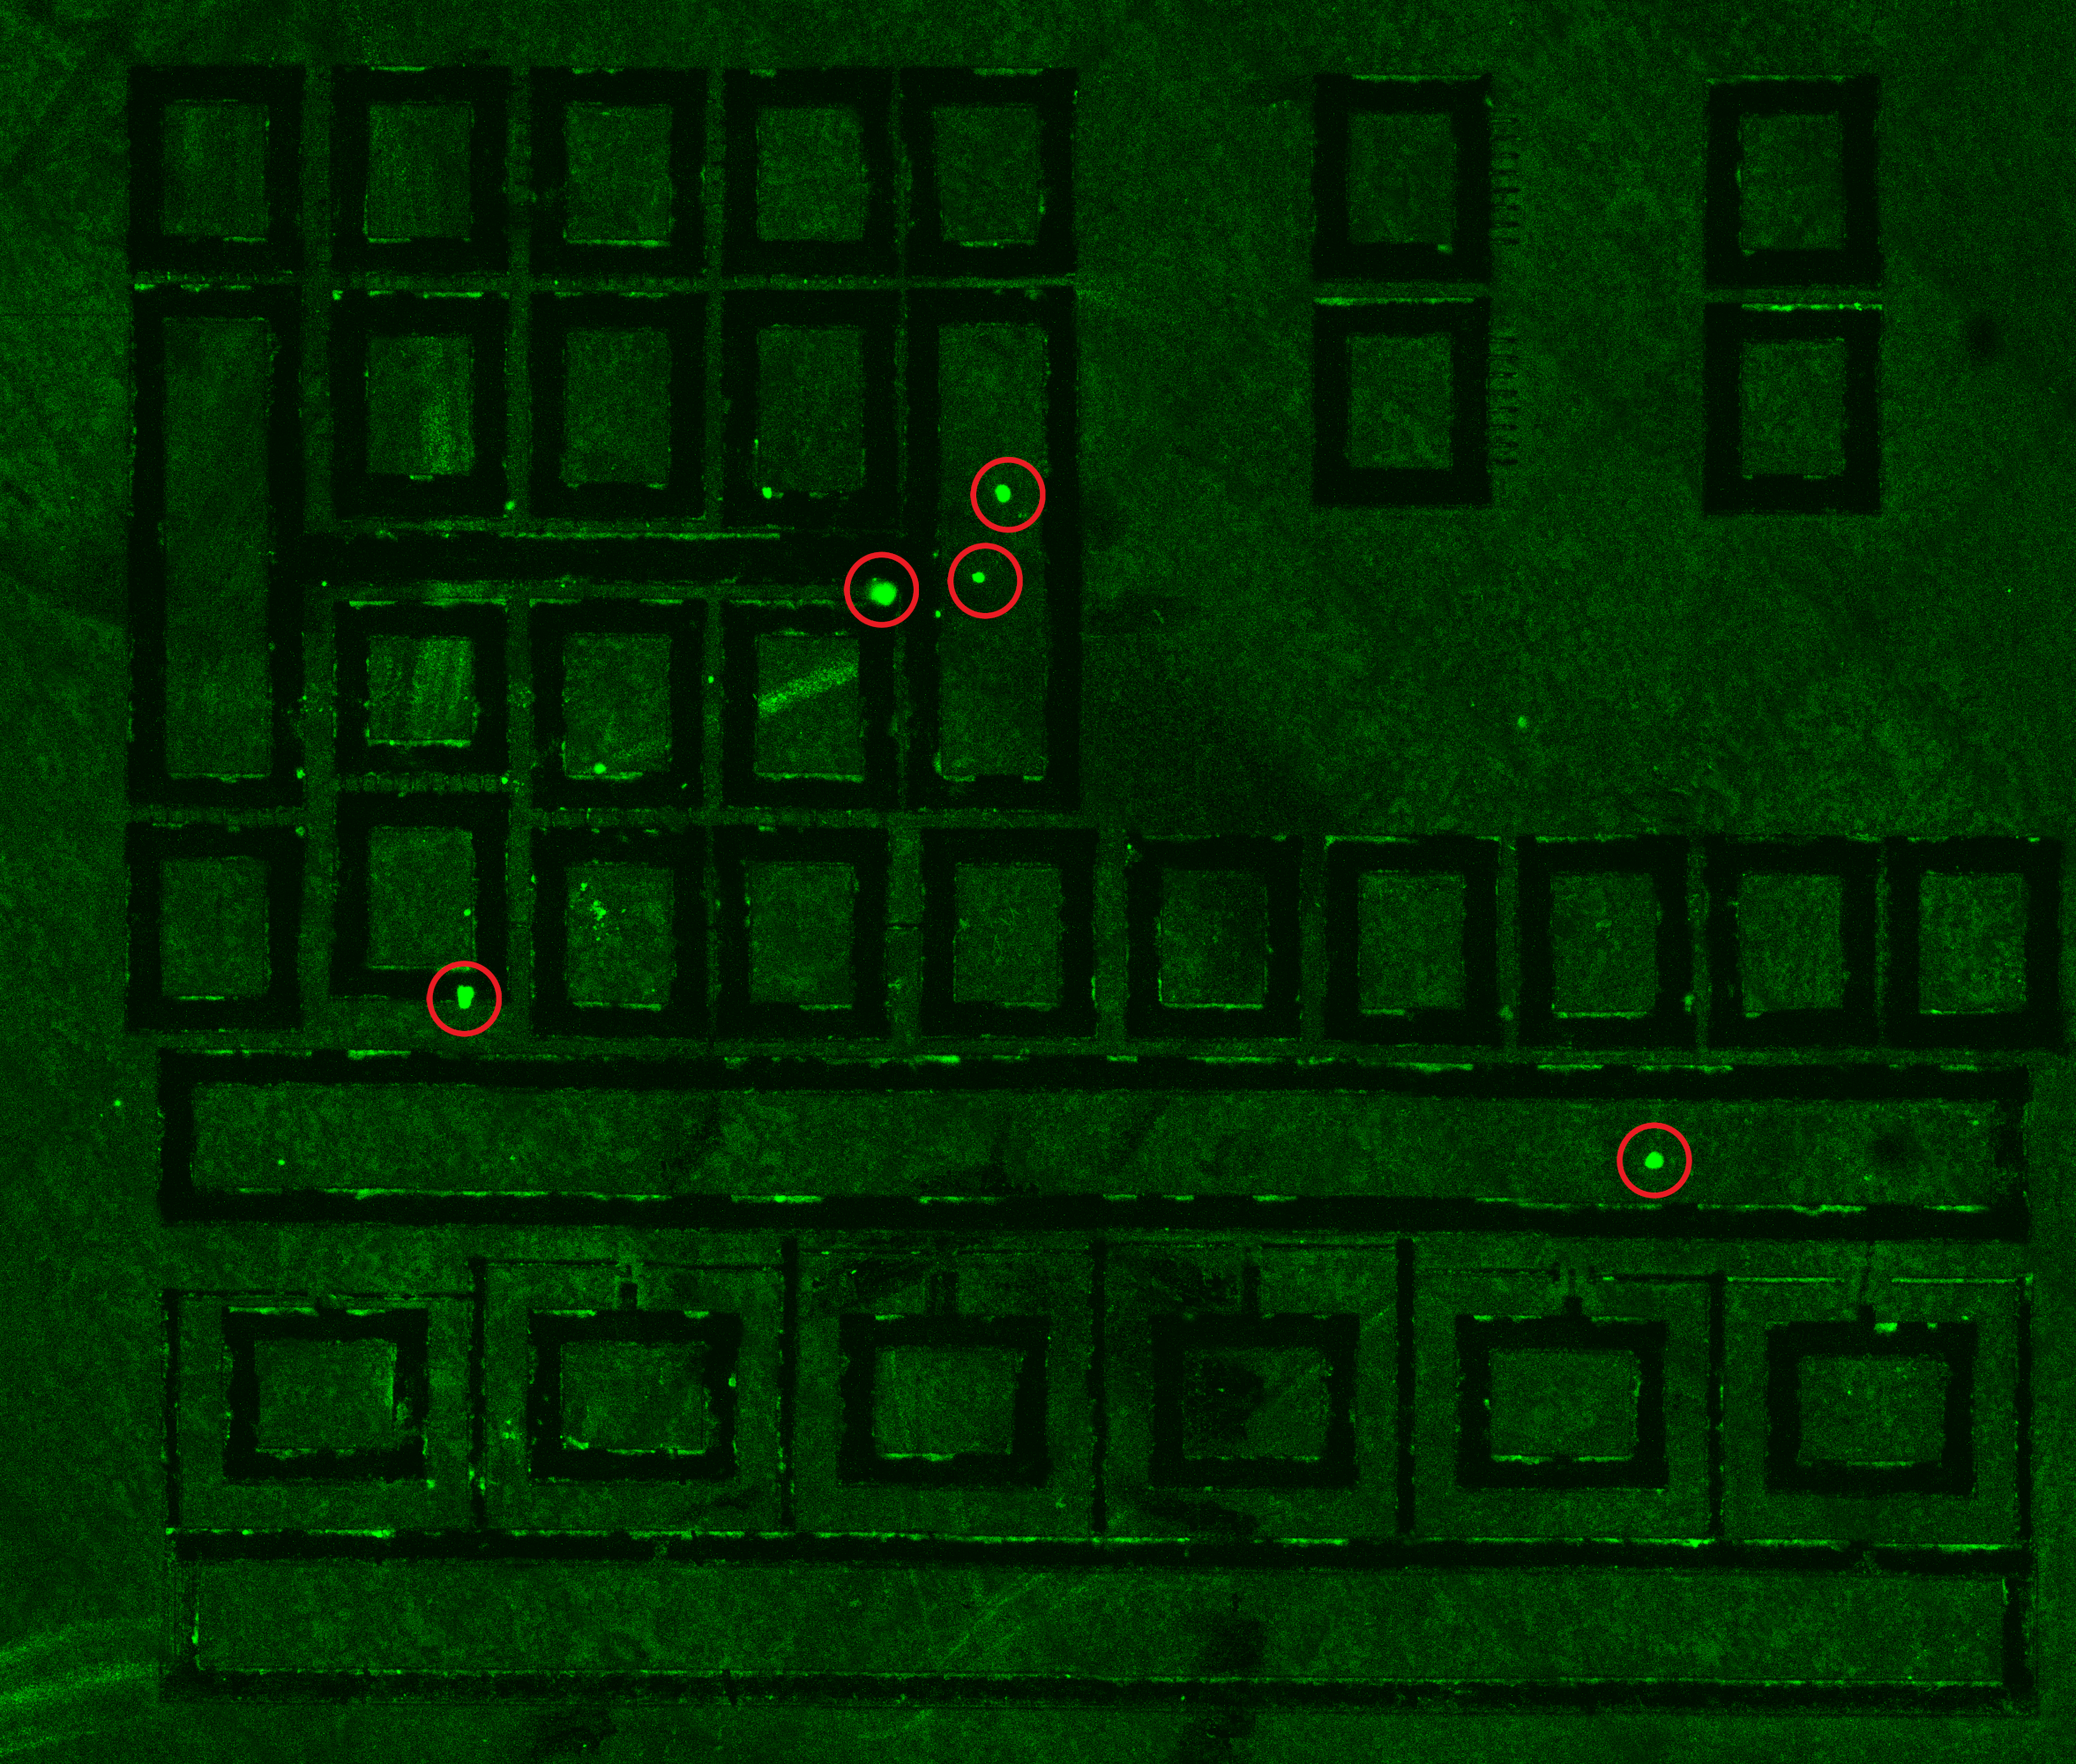
\includegraphics[width=\linewidth]{Chapter7/Figs/Raster/FL_crop 2_low.jpg}
    \caption{A cropped down form of the fluorescent track only, demonstrating the non-uniformity of fluorescence concentrations.}
    \label{fig:fl_crop2}
\end{figure}

Figure \ref{fig:fl_crop2} takes a closer look at the laser processed region of the sample, with only the fluorescence track from the confocal microscopy represented in this image. Note that while the effective spectroscopic analysis of colour filtering did reveal a fluorescence peak in the region of 500--520~\si{\nano\metre}, the green colouration of the fluorescence is a false colour applied to all detected fluorescence used to aid in contrast and the actual colouring may differ. Some fluorescence appears to be present on the surface of the diamond sample, marked by the red circles. In select locations it appears to be on the edge of the laser processed material and yet it is also on the unaltered diamond surface. Due to this inconsistency, it is assumed that this fluorescence is neither due to the substrate or the laser processing, and is likely caused by organic surface contamination despite solvent cleaning steps.

\subsection{Raman Characterisation}
\label{subsec:raman_characterisation}
\begin{table}[ht]
\centering
\begin{tabular}{ccc}
\hline
Position (cm$^{-1}$) & Typical FWHM (cm$^{-1}$) & Assignment \\ \hline
1332                 & 5--10                    & first-order diamond Raman line \\
1355                 & 250                      & $sp^2$ (D peak) \\
1575                 & 100                      & $sp^2$ (G peak) \\ \hline
\end{tabular}
\caption{Raman peaks of interest in diamond and carbon related materials \cite{prawer2004, Tuinstra1970}.}
\label{tab:raman_peaks}
\end{table}

As outlined in section \ref{subsubsec:raman}, raman microscopy provides an effective tool for examining the composition of diamond samples. Table \ref{tab:raman_peaks} summarises the relevant peaks of interest for diamond, with the general deconvolution of CVD diamond raman spectra into a diamond line and the D or G modes of amorphous carbon. The relative intensity of diamond to D or G signals is strongly dependent upon excitation wavelength, with the exact mechanisms behind this likely linked to resonance enhancement of the sp$^{3}$ component and decreasing resonance in the sp$^{2}$ component \cite{prawer2004}. Another noteworthy point on excitation wavelength is that the typical rising background seen with excitation sources such as the green argon ion laser at 514.5~\si{\nano\metre} is commonly attributed to strong photoluminescence from nitrogen-vacancy defects \cite{Filik2005}. The laser wavelengths used can be varied depending upon the application, but background subtraction allows for visible peaks even in the case of high background photoluminescence. A laser wavelength of 532~\si{\nano\metre} was used with the LabRam HR-800 Jobin Yvon at the SAgE analytical facility for the purposes of characterising the laser processed device structures and heavily phosphorous doped surface layer. 

One other relevant consideration for raman spectroscopy of samples which have two components, such as amorphous carbon, is the relative polarisability of the components. $\pi$ bonds formed by sp$^{2}$ hybridised carbons have a higher polarisability than that of the $\sigma$ bonds within sp$^{3}$ hybridised carbon, which results in a larger raman cross-section \cite{Zhang2022}. Additionally, $\pi$ bonds are resonantly enhanced with visible excitation lasers while $\sigma$ bonds are not. This tends to lead to a dominance of sp$^{2}$ signal in samples where even low ($\sim20$\%) fractions of sp$^{2}$ material is present \cite{Ferrari2004}. 
To summarise, for single crystal diamond the position and FWHM of the diamond line, and relative intensity of the diamond line to the G and D peaks are used as crude measures of crystallinity \cite{Bennett2024}. This is due to single crystal diamond only displaying the first order diamond line while grain boundaries in polycrystalline films will produce varying intensities of D and G peaks depending upon the grain sizes \cite{Bachmann1994}. At the extreme of pure graphite, only the crystalline G peak remains, while in all other forms of graphitic materials the disorder D peak appears \cite{Tuinstra1970}. 

\subsubsection{Amorphous Carbon}
Amorphous carbon (a-C) is made up of unstructured mixtures of sp$^{3}$ and sp$^{2}$ hybridised carbon. The properties of such material is dependent upon the ratio of sp$^{3}$ and sp$^{2}$ bonding, with amorphous carbon films of high sp$^{3}$ content forming a harder material which is more transparent and of higher resistivity than of materials with high sp$^{2}$ content \cite{Suzuki20042}. Films of high sp$^{3}$ content are also highly stressed \cite{Marques2000}, and are hence more likely to delaminate from the substrate surface. Amorphous carbon films can also be hydrogenated, which is quite common for CVD grown films \cite{Robertson1996}. These hydrogenated amorphous carbon films are softer, more stable, and will tend to be more transparent than hydrogen-free films. There is also a variable range hopping conduction mechanism between clusters of hydrogenated sp$^{2}$ carbon in amorphous carbon films which may represent a possible conductive path in the case of laser processed diamond \cite{Tomidokoro2021}.

\begin{figure}[H]
    \centering
    \includegraphics[width=\linewidth]{Chapter7/Figs/Raster/raman_both.png}
    \caption{Relative intensities of raman spectra for untreated and laser-treated portions of sample G. The spectra are normalised such that the sp$^{3}$ peak for both examples is set to 1.}
    \label{fig:raman_both}
\end{figure}

\begin{table}[ht]
\centering
\begin{tabular}{cccc}
\hline
Material Type & Raman Shift (\si{\per\centi\metre}) & Relative Intensity & FWHM (\si{\per\centi\metre}) \\ \hline
Non-Processed & 1334 & 1.00 & 2.24 \\ 
Non-Processed & 1554.3 & 0.08 & 63.81\\
Laser Processed & 1333.6 & 0.99 & 2.28 \\
Laser Processed & 1582.2 & 0.12 & 29.53 \\ \hline
\end{tabular}
\caption{Raman spectrum data comparing non-processed and laser-processed materials.}
\label{tab:raman_data_combined}
\end{table}

In figure \ref{fig:raman_both}, two different raman spectra are plotted, which represent a portion of the sample that has been laser processed, and another region which was well away from any laser processing on the phosphorous doped diamond surface. The exact location used for the laser processed region is indicated by the red square in figure \ref{fig:raman_section}, which was chosen due to the large radius of laser processed material that surrounds the centre point. While it is not possible to guarantee that the laser spot will only be absorbed and otherwise interact with the visibly darkened, laser affected region of diamond, this location was chosen to maximise any sp$^{2}$ raman signal. 
\clearpage

\begin{wrapfigure}{r}{0.4\linewidth}
  \centering
  \includegraphics[width=\linewidth]{Chapter7/Figs/Raster/raman_section_anno.jpg}
  \caption{A 488~\si{\nano\metre} confocal microscope image of the raman area, showing the section of the sample under investigation.}
  \label{fig:raman_section}
\end{wrapfigure}

The "Non-Processed" region was strategically chosen on the opposite side of the diamond sample (on the same face with a phosphorous doped surface layer), away from any laser-written areas. However, due to the optical transparency of diamond, it remains a slim possibility that any sp$^{2}$ raman signal from this location may be due to a distant, laser processed portion. 

As shown in figure \ref{fig:raman_both} and table \ref{tab:raman_data_combined}, there is a shift in what may be considered the G peak, rising from a small hump that may be attributable to the highly phosphorous grown surface layer, to a moderate peak in the raman spectra of laser processed material. Both spectra show a small shift in the 1332~\si{\per\centi\metre} diamond peak, and they also have a similar FWHM for this line. While there is a visible difference between these two raman spectra, it is difficult to say that the laser processed material represents highly graphitised material, especially compared to the relative shifts that are typical for laser modified diamond \cite{kononenko1998, kononenko:2008}. However, the rise in G peak does indicate a change in the material structure due to the laser processing, in accordance with a rise in sp$^{2}$ carbon content.

\printbibliography[heading=subbibliography]
\end{refsection}